% Chapter 2

\chapter{Recursive partitioning and ensemble methods} % Chapter title

\label{ch:methods} % For referencing the chapter elsewhere, use \autoref{ch:methods} 


	Recursive partitioning is a non-parametric, data-driven statistical algorithm that iteratively searches a given predictor space to identify potential splits, thus segmenting the space into distinct, rectangular subsections. Then, a simple model, most often a constant, is fit in each one \cite{hastie2009elements}. In the case of a continuous outcome, this recursive partitioning procedure is referred to as a \textit{regression tree}, and the constant reflects the mean value of all observations in a given subsection. Otherwise, if the outcome is categorical, it is referred to as a \textit{classification tree}, and the constant is assigned to be the specific category with the highest frequency over all observations in the particular subsection. As such, recursive partitioning is not limited to a binary outcome, but can actually model an outcome with $K$ potential classes.


	This framework was initially formulated through the seminal work of \citeA{morgan1963problems}, who proposed focusing on predictive accuracy in large survey data as a means to relax additive assumptions commonly made at that time in order to detect complex relations among predictor variables; a process they referred to as Automatic Interaction Detection. This framework was further solidified by both \citeA{breiman1984classification} and \citeA{quinlan1986induction}, who created algorithms seeking to improve on this original idea. Initially, recursive partitioning was met with much disdain by the statistics community due to its poor generalizability, especially when inappropriately applied to small data sets with large noise-to-signal ratios \cite{hastie2013}. However, this recently changed in the past decade or two, when the work of \citeA{breiman1984classification} started to become widely adopted as a useful tool in predictive modeling. Still, this method is relatively unknown to those in the social sciences \cite{mcardle2013}.


	Given the immense popularity of the recursive partitioning framework, it is no surprise that many algorithms exist, each with their own advantages and disadvantages. This dissertation focuses on two of the most widely used recursive partitioning algorithms: classification and regression trees \cite<CART;>{breiman1984classification} and conditional inference trees \cite<CTREE;>{hothorn2006unbiased}. These two algorithms, in addition to other important concepts inherent in predictive modeling, are described below. To assist in this overview and to highlight how the methods are used in practice, a data set examining the relation between graduation rates and various statistics for US Colleges (N = 777) from the 1995 issue of US News and World Report will be used. This data set is freely available from the ISLR package \cite{ISLRR} in the R software environment \cite{Rcore}, and contains 17 variables that can be used as predictors for graduation rate, such as whether a university is private or public, the acceptance rate, and the out-of-state tuition cost. 


%----------------------------------------------------------------------------------------

\section{Classification and regression trees}


	Originally proposed by \citeA{breiman1984classification}, CART is easily the most popular and widely used recursive partitioning algorithm, being cited almost 26,000 times according to Google Scholar\footnote{As of November 13, 2014}. When initially creating a decision tree, the algorithm consists of essentially four steps \cite{james2013introduction}. First, all predictor variables are initially considered for potential splits in a \textit{greedy}, \textit{top-down} manner. The splitting process is greedy, because each step searches for the best possible split at that time, rather than considering previous or future steps. It is top-down, because it begins with all observations belonging to the same group, or node, and then subsequently conducts splits further down the tree after initial splits have been made. Second, the best potential split is identified by some criterion, which is taken to be the residual sums of squares (RSS) in the case of a continuous outcome. Following the notation of \citeA{hastie2009elements}, suppose we have a predictor variable $X_j$ with a given split point $s$, which splits the predictor space into two regions: $R_1(j, s) = \left\{ X \mathrel{}\middle|\mathrel{} X_j < s\right\}$ and $R_2(j, s) = \left\{ X \mathrel{}\middle|\mathrel{} X_j \geq s\right\}$. The algorithm searches for a particular $j$ and $s$ that minimizes the following equation:

\begin{equation} 
\sum_{i: x_i \in R_1(j, s)} (y_i - \hat{y}_{R_1})^2 + \sum_{i: x_i \in R_2(j, s)} (y_i - \hat{y}_{R_2})^2
\end{equation}

\noindent where $\hat{y}_{R_j}$ is the mean of the outcome within the $j$th subsection and $\sum_{i: x_i \in R_j(j, s)} (y_i - \hat{y}_{R_j})^2$ is the RSS over all $i$ participants in the $j$th subsection.

	Once the best split is identified, the data is split on this threshold, creating two new subsections, or \textit{child nodes}. The same procedure outlined above is then performed separately on each of these nodes, and this process is repeated until some stopping criterion is reached. For example, the algorithm might require a minimum number of observations to belong to a given node, regardless of whether another split will result in a reduction of the RSS. Finally, the given node becomes a \textit{terminal node} once no further splits can be made within that node. When all nodes can no longer be split any further due to these stopping criteria, the algorithm terminates. 

	See \autoref{fig:exampletree} for an example decision tree might look in the college graduation rate data set. The corresponding decision tree first splits on the out-of-state tuition variable, which is a variable reflecting the annual tuition cost a student has to pay to attend the institution when they live in a different state (range: \$2340 - \$21700). This decision creates a vertical line in two-dimensional space, splitting the data into two subsections at approximately \$10,000. Both of these nodes are again split by the out-of-state tuition variable, resulting in two more lines being drawn and creating four subsections in total. Finally, one node is further split by the percentage of students at an institution who were in the top ten percent of their high school class, resulting in a horizontal line creating a fifth subsection. Note that only two variables were used in the splitting process to maintain interpretability with the corresponding visualization.


\begin{figure}
\begin{tabular}{c}
\subfloat[]{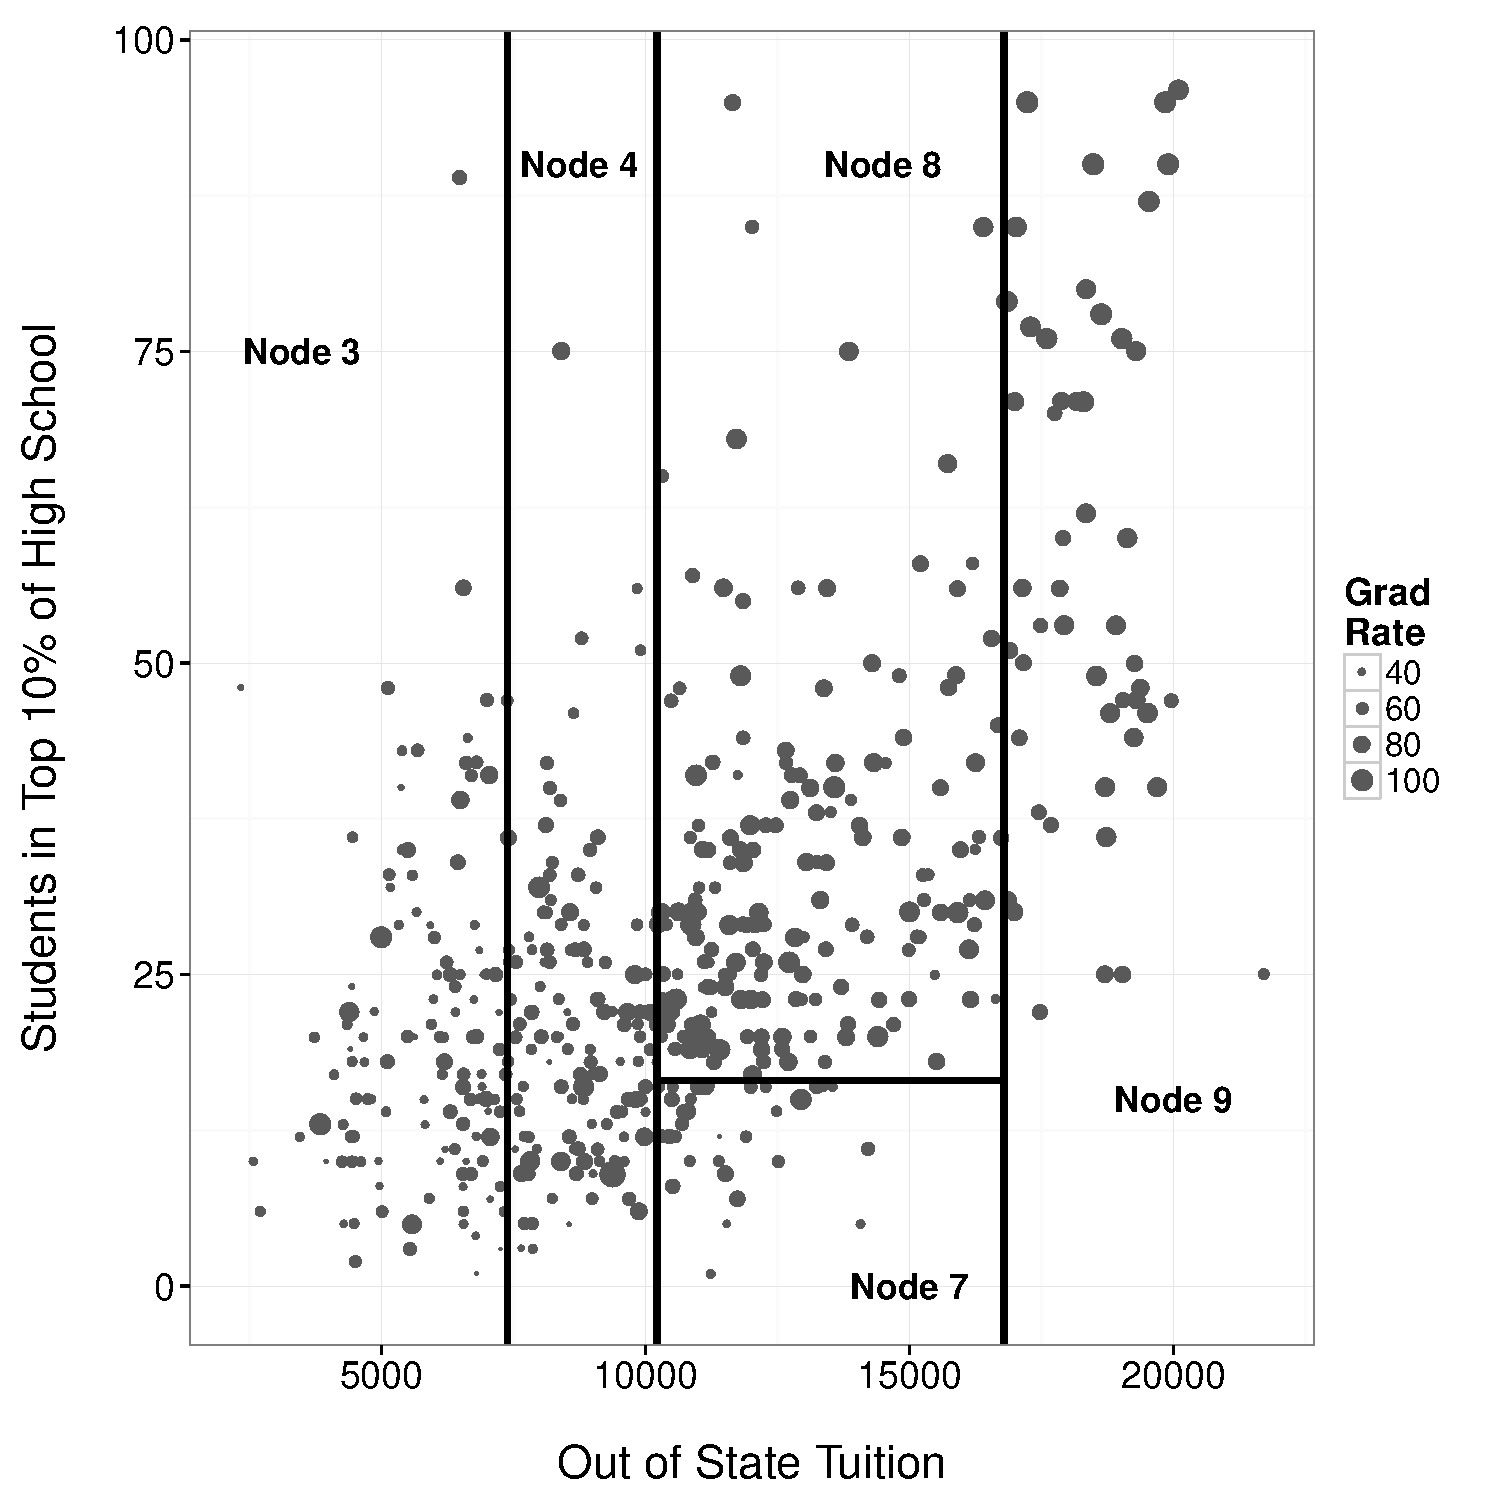
\includegraphics[width = 3.5in]{Figures/Chapter02/part_plot.pdf}} \\
\subfloat[]{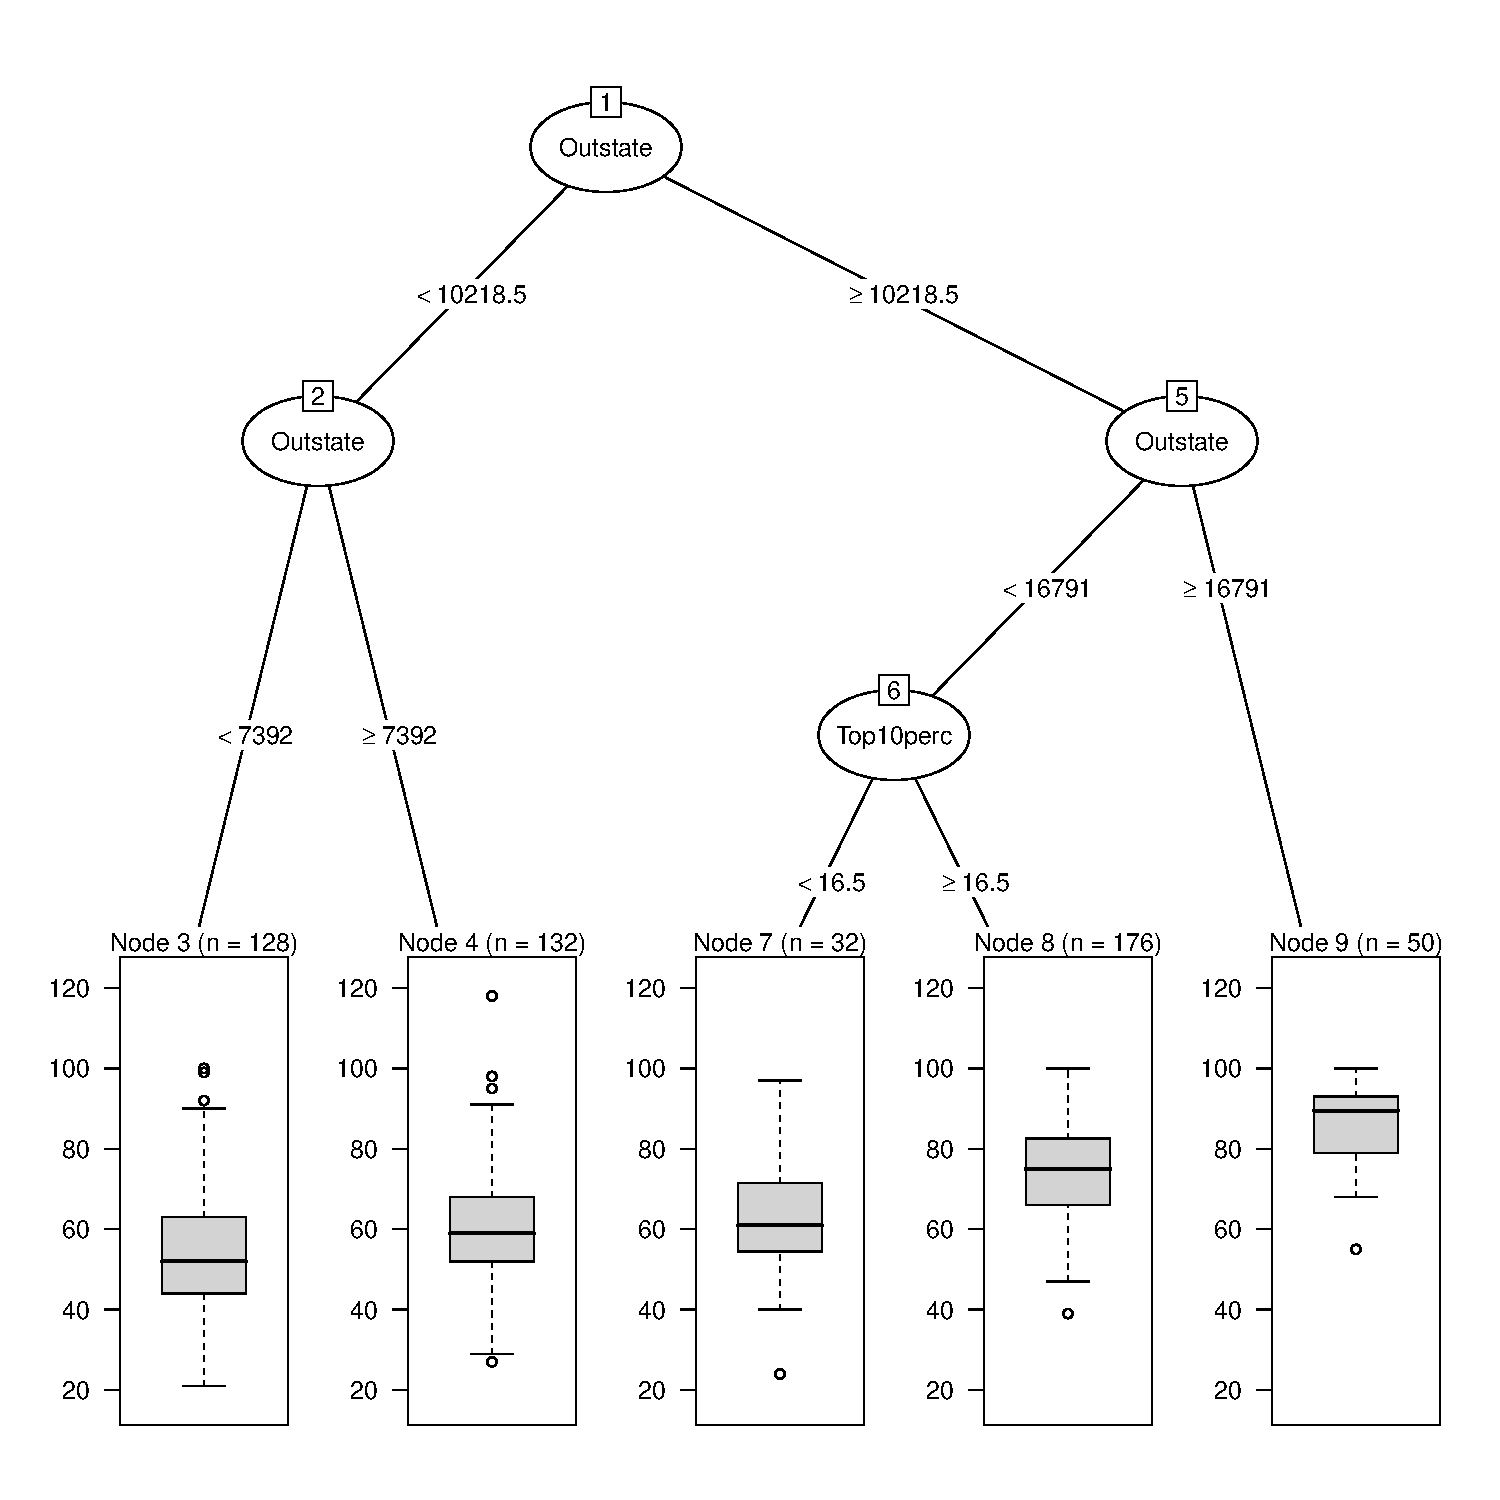
\includegraphics[width = 3.5in]{Figures/Chapter02/example_tree.pdf}} 
\end{tabular}
\caption[An example decision tree.]{\textit{(a) shows how college graduation rates vary as a function of out-of-state tuition and percentage of students in the top 10\% of their high school class. These partitions are created by a set of binary decision rules, shown in (b).}}
\label{fig:exampletree}
\end{figure}


%----------------------------------------------------------------------------------------

\subsection{Understanding the bias-variance tradeoff}


	In the previous example, we see the last split results in a subsection with a small sample size ($N = 32$). When growing a decision tree on an initial data set, referred to as the \textit{training set}, creating a tree with more depth and complexity will yield excellent performance. However, because of the subtleties in the data at hand, the same tree is likely to have poor performance generalizing to independent data. In other words, the tree algorithm is \textit{overfitting} the data. This highlights the importance of validating a decision tree (or any predictive model for that matter) on a separate data set, referred to as the \textit{test set}, to get a more accurate estimation of its generalizability.


	The underlying reason overfitting occurs is due to the \textit{bias-variance tradeoff}. Conceptually, bias refers to the difference between a true value and the average prediction of said value over many sample data sets drawn from the same population. Variance, on the other hand, refers to how much variability exists in your predictions for a given data point. Models of low complexity typically have high bias and lower variance, while models of high complexity typically have low bias and high variance. Overfitting occurs when your model has too much variance due to being overly complex, resulting in predictions that generalize poorly to new data \cite{hastie2009elements}. Thus, this bias-variance tradeoff is a balance between trying to identify a model with low bias that is still parsimonious enough to perform well on new data. Refer to \autoref{fig:tradeoff} to see how predictive performance varies as a function of model complexity between a training set and a test set in the graduation rate data. As the predictive model becomes more complex (i.e., more splits in the case of a decision tree), the estimated error always improves in the training set, but only improves to a certain extent in the test set. In this case, there is evidence for overfitting when the decision tree contains more than three or four splits. 


\begin{figure}[h]
  \centering
  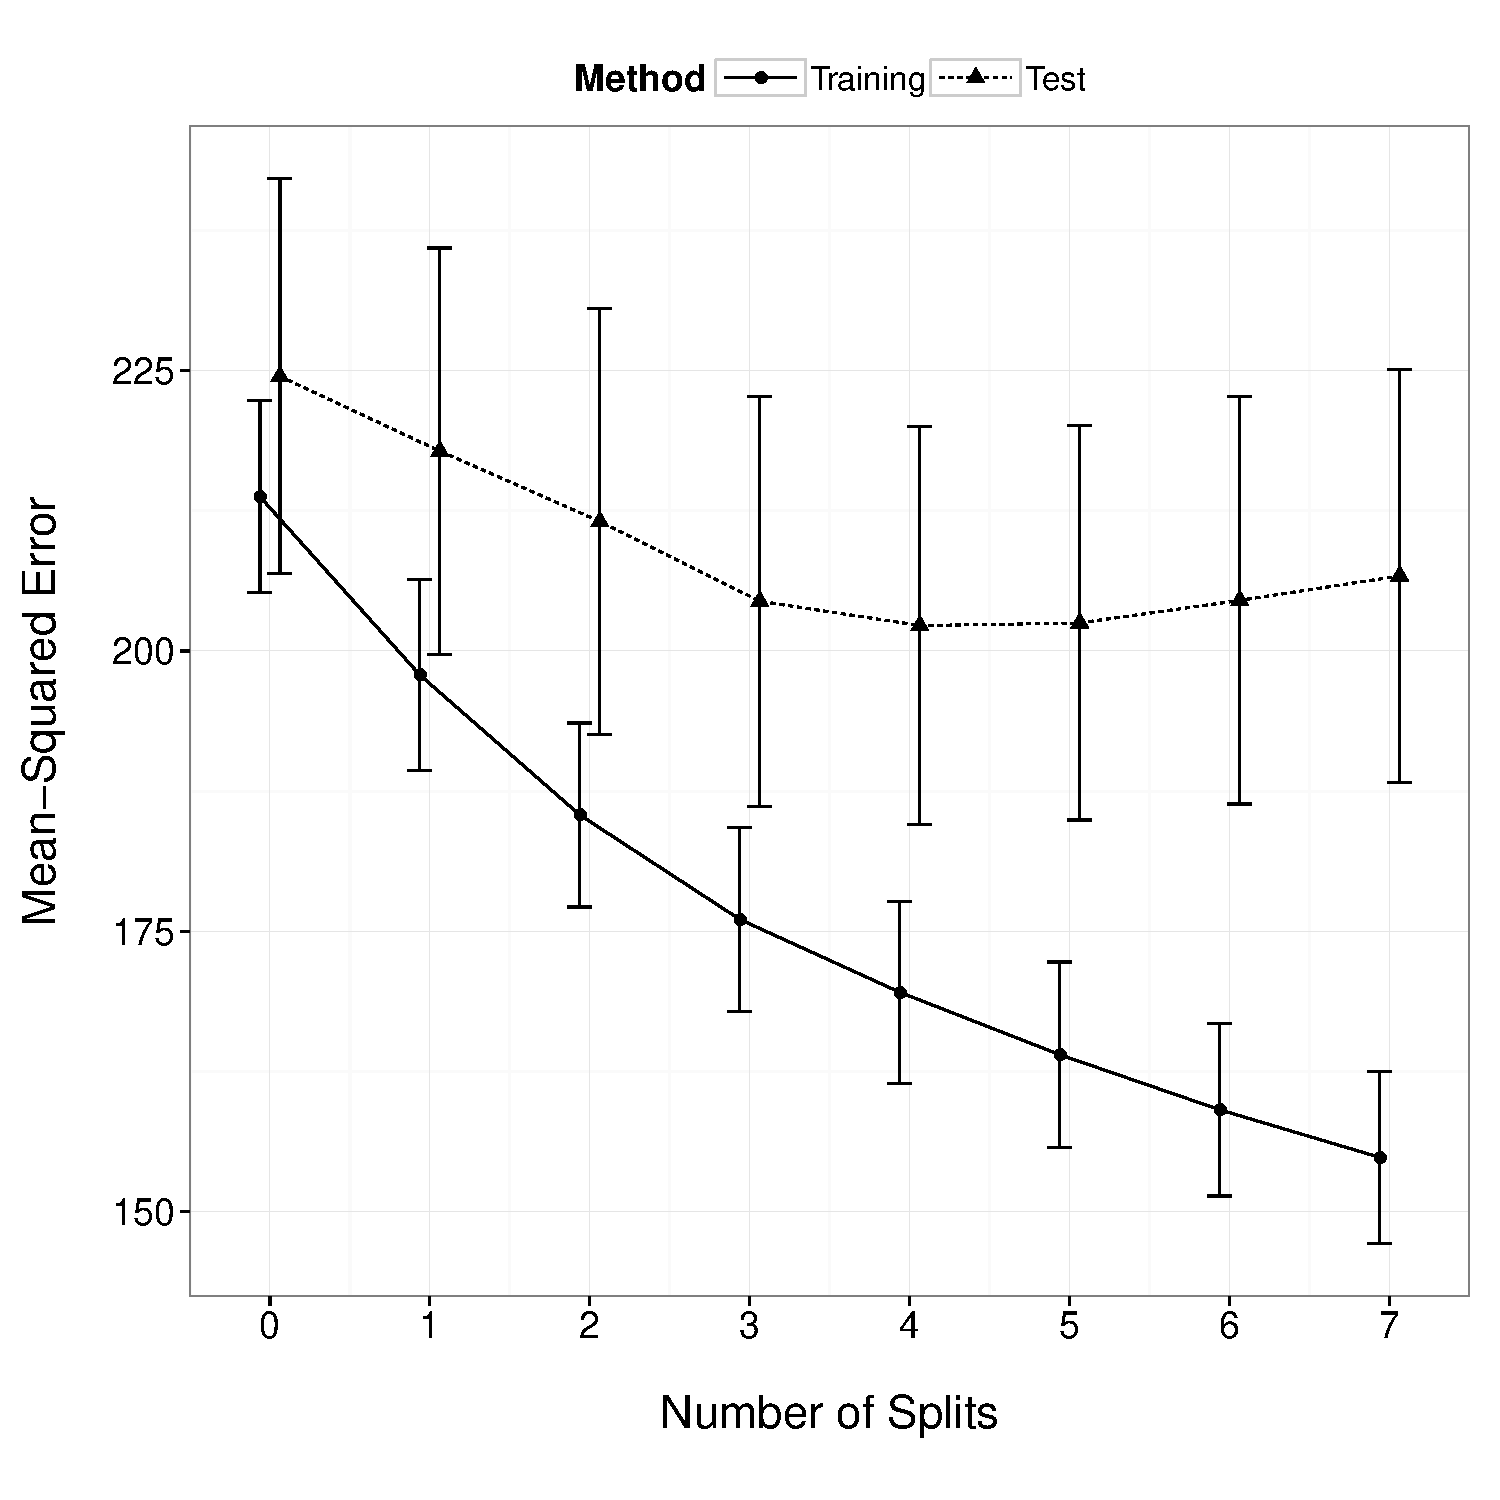
\includegraphics[width=3.5in]{Figures/Chapter02/bias_var_plot.pdf}
  \caption[The bias-variance tradeoff in the graduation rate data.]{\textit{The bias-variance tradeoff found in the graduate rate data, depicting how the error changes as a function of model complexity. The data was split into training and test sets 100 times to estimate precision, and the bars represent 1 standard error. Note that this figure was inspired by \cite{james2013introduction}.}}
  \label{fig:tradeoff}
\end{figure}


	The bias-variance tradeoff can also be understood mathematically as a decomposition of the residual term in a given statistical model. Given a training set consisting of data points $x_i, \ldots, x_n$, each with a corresponding $y_i$, we can assume there exists some true functional relationship, $y_i = f(x_i) + \epsilon$, where $\epsilon$ is a noise term with a mean of zero and variance $\sigma^2$. By choosing some statistical method, say linear regression, we get an estimate of $f(x)$, namely, $\hat{f}(x)$. The total squared error of this estimated function relation can then be defined as:

\begin{equation}
\begin{aligned}
\mathbb{E}[(y - \hat{f}(x))^2] &= \mathbb{E}[(f(x) - \mathbb{E}[\hat{f}(x)])^2] + \mathbb{E}[(\hat{f}(x) - \mathbb{E}[\hat{f}(x)])^2] + \mathbb{E}[\epsilon^2] \\
&= Bias(\hat{f}(x))^2 + Variance(\hat{f}(x)) + \sigma^2
\end{aligned}
\end{equation}


%----------------------------------------------------------------------------------------

\subsection{Pruning decision trees with cross-validation}


	Because decision trees that are too complex typically yield poor generalization performance, an additional step must be introduced into the process of building and evaluating a decision tree. How this issue is typically handled is with a procedure known as \textit{pruning}. That is, trees are initially grown out to their maximum depth (i.e., maximum complexity) with the algorithm outlined above. Then, the depth of the tree is reduced based on a given cost function. For any subtree $T$ that is a subset of a decision tree grown to full length, define $|T|$ as the number of terminal nodes in $T$, and $\alpha \geq 0$ as the complexity parameter. The updated cost-complexity measure, $RSS_{\alpha}(T)$, can be given as


\begin{equation}
RSS_{\alpha}(T) = RSS + \alpha|T|
\end{equation}


\noindent Here, the complexity parameter can be tuned to control how complex the resulting tree is. If $\alpha = 0$, no pruning will be done. When this value increases, however, the depth of the tree will get smaller. 

	The cost complexity parameter only has a finite number of values, because there is only a finite number of subtrees within a given tree. Once all the alpha values corresponding to unique subtrees have been collected, the value correponding to the best performance is selected with a procedure known as \textit{k-fold cross-validation}. This procedure first divides the training set into $K$ equal-size partitions, or folds. First, a full tree is grown on all but the $k$th fold. The mean squared error is then extracted from the left-out $k$th fold as a function of the complexity parameter. This procedure is repeated $K$ times, so every partition has an opportunity to act as a test set. The complexity parameter value that leads to the lowest average error across the $K$ estimates is chosen for the creation of the final tree to be used for future predictions. Note that setting $K$ as five or ten yields a good approximation to the true test error in many applications, so these values for $K$ are typically chosen \cite{hastie2009elements}. Another rule of thumb for selecting the value of the complexity parameter is known as the \textit{1-SE rule} \cite{breiman1984classification}. Because the cross-validation estimate of the complexity parameter results in a distribution of error estimates, the value of the complexity parameter is selected such that the simplest tree within one standard error of the best tree is chosen. 
	

	\autoref{fig:pruning} shows how the 1-SE rule is applied in practice for the college graduation rate data set. Recall that \autoref{fig:tradeoff} indicated that three or four splits should be made, while the 1-SE rule indicates only one split should be made. This highlights a feature of the 1-SE rule, in that it typically selects more parsimonious models, which may or may not yield better generalization performance. Thus, the result of the 1-SE rule should be compared with other evidence, like \autoref{fig:tradeoff}, to help determine how best to prune a decision tree. 


\begin{figure}[h]
  \centering
  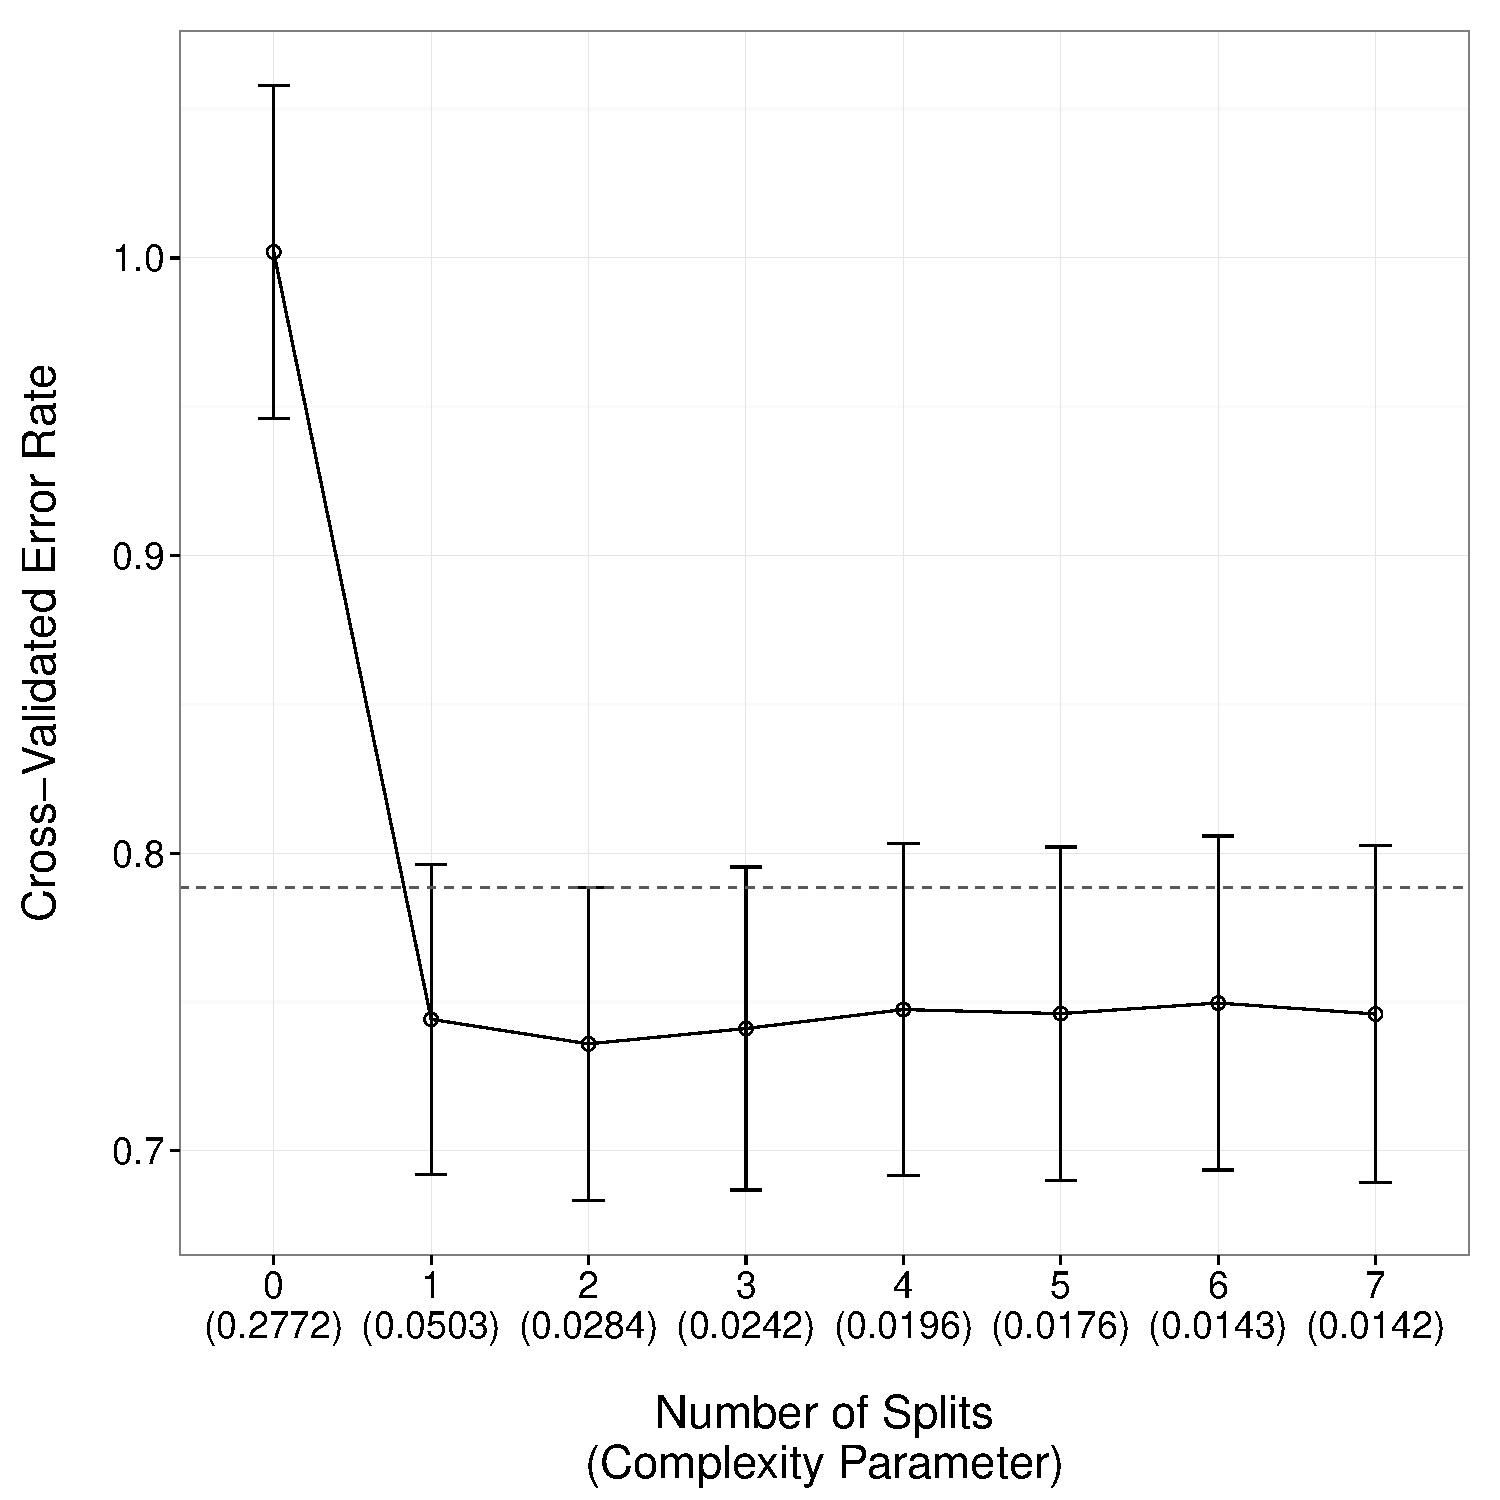
\includegraphics[width=3.5in]{Figures/Chapter02/cp_plot.pdf}
  \caption[Using cost-complexity pruning on the graduation rate data set.]{\textit{How the 10-fold cross-validation error changes as a function of model complexity in the college graduation rate data set. The 1-SE rule is set with the dotted line, indicating that this rule of thumb would select one split. Just selecting the tree that yields the minimum cross-validated error would select a tree with two splits.}}
  \label{fig:pruning}
\end{figure}


%----------------------------------------------------------------------------------------

\subsection{CART with a categorical outcome}

	While not discussed in the introduction to CART above, the algorithm can easily be extended to a categorical outcome with K potential classes by simply modifying the RSS criteria for both the splitting and pruning. More specifically, three methods exist as a measure of node purity in the case of a categorical outcome: classification error, the Gini index, and cross-entropy. Classification error is the simplest of the three, and is the fraction of observations in the training set that do not belong to the most common class


\begin{equation}
Classification \ error = 1 - \max_k(\hat{p}_{jk})
\end{equation}


\noindent where $\hat{p}_{jk}$ corresponds to the proportion of observations in the training set in the $j$th subsection that are from the $k$th class. While the classification error rate only includes the most common class, the Gini index reflects a measure of total variance across all possible classes


\begin{equation}
Gini = \sum_{k=1}^{K}\hat{p}_{jk}(1 - \hat{p}_{jk})
\end{equation}


\noindent Finally, cross-entropy is numerically similar to the Gini index, and is defined as


\begin{equation}
Entropy = -\sum_{k=1}^{K}\hat{p}_{jk}log(\hat{p}_{jk})
\end{equation}


	The relation between these three measures can be seen in \autoref{fig:compare_cat}. When the probability of belonging to a class in a given node becomes more certain (i.e., closer to 0 or 1), the values of all three measures get closer to zero. Otherwise, when the probability of an observation belonging to a specific class gets more uncertain (i.e., closer to 0.5), the value of these measures increase. In other words, these measures calculate how homogenous a given node is, and the goal of the recursive partitioning algorithm is to minimize this value over all nodes in the splitting process. Note that either the Gini index or cross-entropy are typically favored in the splitting process, as they are more sensitive to node purity when compared with the misclassification rate \cite{james2013introduction}. If the probabilities of a given class are small, cross-entropy is likely a better choice compared with the Gini index, because of the log in the calculation. However, research has found no conclusive evidence regarding whether the Gini index or cross-entropy yields better performance in a general sense \cite{raileanu2004theoretical}.


\begin{figure}[h]
  \centering
  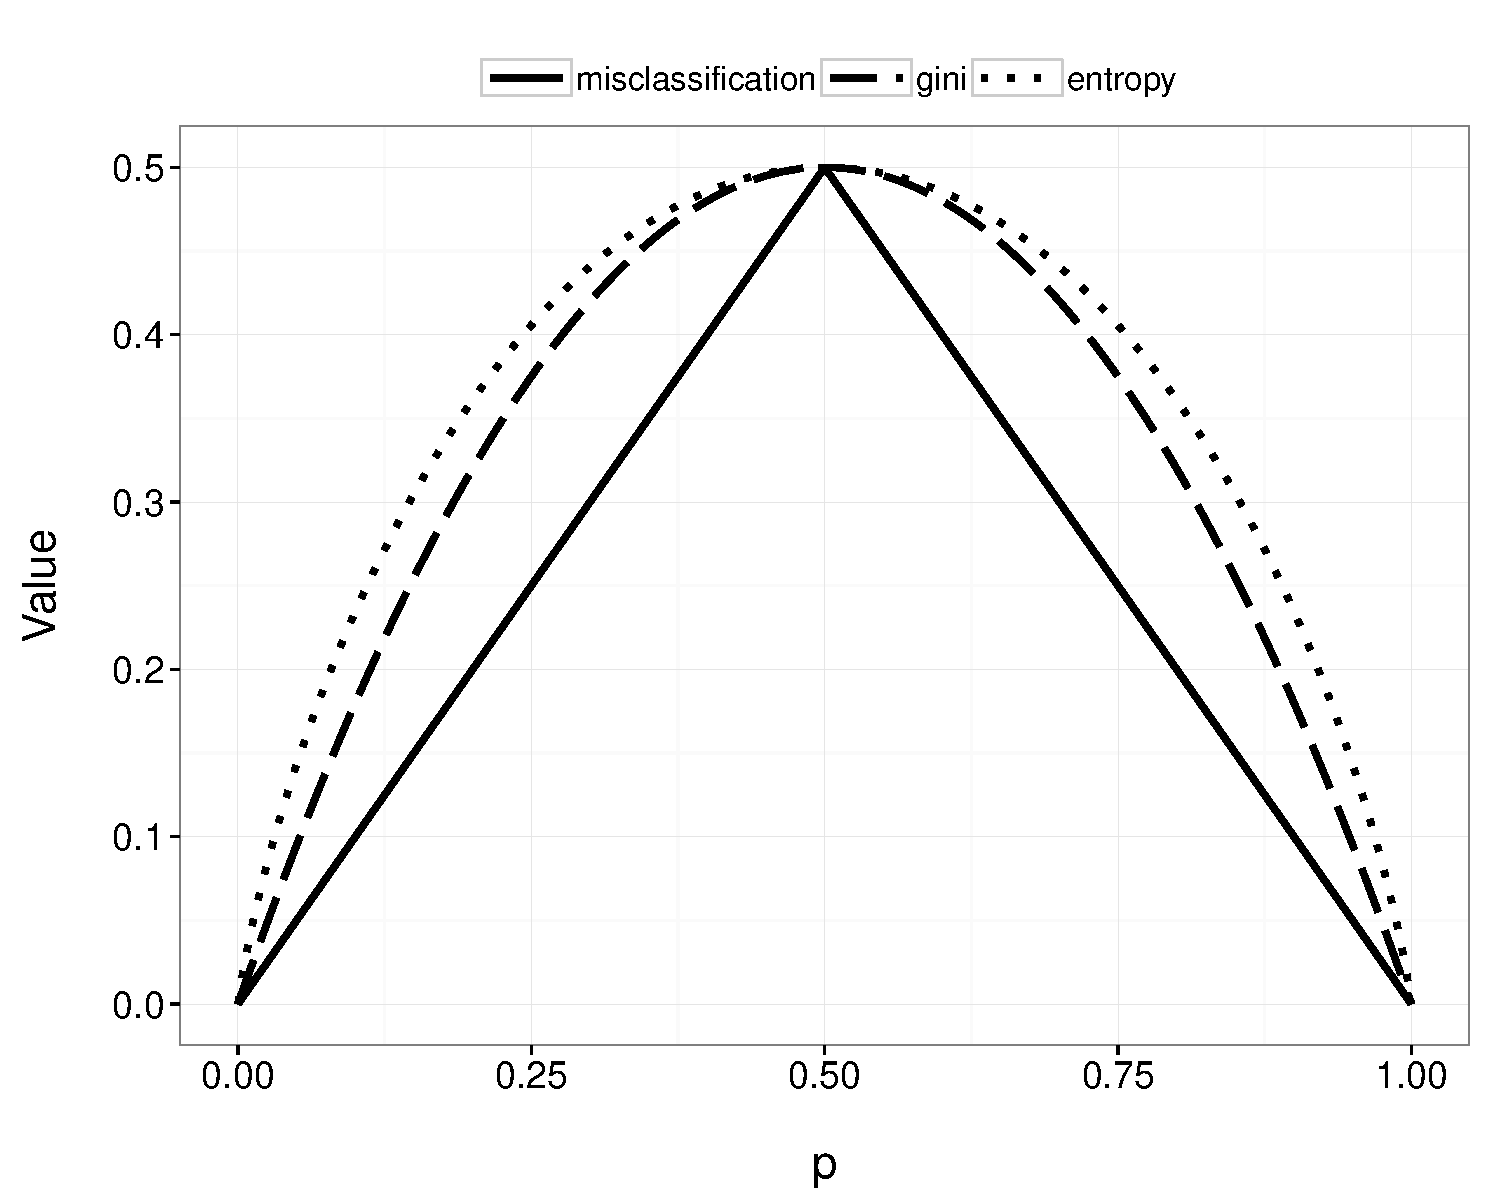
\includegraphics[width=3.5in]{Figures/Chapter02/compare_cat_long.pdf}
  \caption[The relation between classification error, the Gini index, and cross-entropy.]{\textit{The relation between classification error, the Gini index, and cross-entropy at different probability values for belonging to a given class when two classes are present. Image adapted from \cite{hastie2009elements}.}}
  \label{fig:compare_cat}
\end{figure}



%----------------------------------------------------------------------------------------

\subsection{Pros and cons of CART}


	CART is a method that can efficiently search a parameter space, capturing potential non-linear relations as well as higher-order interactions without explicit model specification by the researcher. It can also handle both continuous or categorical variables as outcomes by simply changing the underlying measure of node purity. Finally, and perhaps the most relevant to this dissertation, is that the resulting pruned tree is fairly easy to understand and explain to others, even if those individuals are not familiar with the technique or lack a formal statistical background.


	Despite all these advantages, CART is not without drawbacks. First, like all simple decision trees, they generally do not yield good predictive performance when compared to other regression-based techniques \cite{james2013introduction}. Pruning can also add a layer of researcher subjectivity in deciding how complex or simple a given tree is. Finally, because the splitting procedure considers all possible splits within all possible variables simultaneously, variables with more potential splits are more likely to be chosen to have a potential split point purely due to chance when compared with variables with less potential splits \cite{loh1997split, quinlan1995oversearching}. For example, there are $N - 1$ potential splits for a continuous variable (assuming no identical values among observations) and $2^{K - 1} - 1$ potential splits for categorical variables with $K$ categories. Assuming a sample size of 100, a continuous variable with no repetitive numbers or a categorical variable with five classes will have 99 and 624 potential splits respectively, while a 5-point Likert scale item or a dichotomous variable will have substantially less (4 and 1, respectively).


%----------------------------------------------------------------------------------------

\section{Conditional inference trees}


	To mitigate the issue of pruning and the biased splitting procedure found in many recursive partitioning algorithms, \citeA{hothorn2006unbiased} proposed conditional inference trees (CTREE). While conceptually similar to CART, CTREE is based on a well-defined theory of permutation tests developed by \citeA{strasser1999asymptotic}. Like CART, CTREE also consists of four main steps, which will first be explained conceptually. First, a global null hypothesis of independence between $Y$ and all covariates $X_j$ is tested. For a common example, if all covariates and the outcome are continuous, a Pearson's correlation coefficient with a corresponding p-value is calculated for each variable's association with the outcome. If no p-value is below the pre-selected alpha level after accounting for multiple significance tests, the global null hypothesis is not rejected and the algorithm terminates. Otherwise, the covariate with the stongest association (i.e., p-value) with the outcome is selected for splitting. The best split within this covariate is selected, and the training set is partitioned on this value. Finally, these steps are iteratively repeated until the global null hypothesis can no longer be rejected in all subsections. 

	These four steps can also be explained mathematically following notation from \citeA{hothorn2006unbiased} and \citeA{molnar2013}. 

\vspace{8ex}

\noindent Step 1: The Global Null Hypothesis Test \\

First, in a given sample, assume there exists a response $Y$ and a covariate vector $X = (X_1, \ldots, X_p)$. Let $D(Y|X)$ represent the conditional distribution of response $Y$ given the covariates $X$, and $L_n$ represent the training set, such that $L_n = [Y, X_1, \ldots, X_p]$. The global null hypothesis is then defined as $H_0 = \bigcap_{j=1}^{p}H_0^j$, where $H_0^j: D(Y|X_j) = D(Y)$. This is tested with the following test statistic. 


Let $g_j$ be a transformation of the covariate $X_j$, such that $g_j:X_j \rightarrow \mathbb{R}^{p_j}$, where $p_j$ is the number of dimensions the covariate $X_j$ is transormed into. The \textit{influence function}, $h$, performs a similar transformation on the outcome, such that $h: y \rightarrow \mathbb{R}^q$. Also, let $w$ correspond to a set of weights indicating whether a given observation is in a node or not (i.e., set at 1 or 0). The test statistic for every covariate $j$ can be defined as\footnote{Note that this notation differs slightly from \citeA{hothorn2006unbiased}, where $h(Y_i)$ is written as $h(Y_i, (Y_1, \ldots, Y_n))^T$. This was removed for simplicity.}

\begin{equation}
\label{eq:teststat}
T_j(L_n, w) = vec\left ( \sum_{i=1}^{n}w_ig_j(X_{j,i})h(Y_i)^T \right ) \in \mathbb{R}^{p_jq}
\end{equation}


\noindent where the resulting $p_j \times q$ matrix is converted into a $p_jq$ column vector using the $vec$ operator. Note that this final conversion is not a necessity, but is done for computational simplicity. 


 Both the transformation and influence function are chosen depending on the scales of $X_j$ and $Y$, respectively. An outline for selecting both $g$ and $h$ can be found in \citeA{hothorn2006unbiased}. In the frequent case of a numeric variable for both covariate and outcome, both functions can be the identity, indicating that no transformation is made. In the case of a categorical variable, the transformation for said variable can map the covariate into a variable with the number of dimensions equal to the number of categories (i.e., two dimensions in the binary case, with $(1, 0)^T$ for one condition and $(0, 1)^T$ for the other). 


Because the distribution of $T_j$ under the null hypothesis is unknown for most instances, it must be estimated via a \textit{permutation test} framework. That is, a null distribution is contructed by fixing the covariate values and permuting the outcome to destroy the relationship between the covariates and the outcome. The derivation of the conditional expectation $\mu_j$ and covariance $\Sigma_j$ under the null can be found in \citeA{hothorn2006unbiased}, and are not included here for brevity.

With the conditional expectation and covariance, $T \in \mathbb{R}^{pq}$ can be standardized. Let $t$ be the value of $T$, $\mu$ be the expected value of $T$ and $\Sigma_{kk}$ is the $k$th diagonal entry of the covariance matrix under the null distribution. Using these, the maximal entry of $T$ after standardization is chosen for a test statistic $c$:

\begin{equation}
\label{eq:stdteststat}
c(t, \mu, \Sigma) = \max_{k=1,\ldots, pq}\left | \frac{(t - \mu)_k}{\sqrt{\Sigma_{kk}}}  \right |
\end{equation}


The test statistic for each variable, $c(T_j(L_n, w), \mu_j, \Sigma_j)$, is then converted to a p-value scale in order to test the global null hypothesis and for the purpose of variable selection. To reiterate the most recent steps incorporating the permutation test, all observations in a given subsection are randomly permuted, and $c$ is calculated for each covariate. The resulting permuted distribution for a given variable then corresponds to the null distribution assuming no relationship between that variable and the outcome, and a p-value can be calculated as the proportion of the null test statistic distribution that is larger in magnitude than the observed test statistic. The p-values for each variable are corrected for a global test using a multiple comparisons procedure (e.g., Bonferroni), and then compared to the preset $\alpha$ level which is typically (and arbitrarily) defined to be 0.05. If the global test is not rejected, the algorithm makes this node a terminal node. 

\vspace{2ex}

\noindent Step 2: Variable Selection \\


If the global test is rejected, then the variable with the lowest p-value calculated in Step 1 is selected for splitting.

\vspace{3ex}

\noindent Step 3: Split Point Selection \\

Once the variable has been selected, splits are determined using a special case of the test statistic formula defined in \autoref{eq:teststat}. For a selected variable, $X_j*$, the equation is 

\begin{equation}
T_{j*}^A(L_n, w) = vec\left ( \sum_{i=1}^{n}w_iI(X_{j*,i} \in A)h(Y_i)^T \right ) \in \mathbb{R}^q
\end{equation}

\noindent where A is a possible partition of the current observations and

\begin{equation}
I(X_{j,i} \in A) = \left\{
     \begin{array}{rr}
       1 & : X_{j,i} \in A \\
       -1 & : X_{j,i} \notin A
     \end{array}
   \right.
\end{equation}

Note that the values are coded as 1 and -1 so if a given covariate is independent of the outcome, the corresponding values will typically cancel and yield a value for $T_{j*}^A$ that is close to zero.

As defined, this sequence will test all possible subsets of $A$. To reduce the amount of computation, possible subsets for continuous and ordinal variables are restricted to maintain their order among observations. An additional contraint can be made by requiring a minimum node size for all groups within a given subset. Finally, a partition, $A^*$, is identified as the one which maximizes the standardized test statistic using \autoref{eq:stdteststat} with the proposed new split $A$. That is,

\begin{equation}
A^* = \underset{A}{\operatorname{argmax}} \ c(t_{j*}^A, \mu_{j*}^A, \Sigma_{j*}^A)
\end{equation}

\vspace{1ex}

\noindent Step 4: Repeat \\

The weights within each node are re-normalized, and these steps are repeated until the global null hypothesis is no longer rejected in each subsection.


\vspace{2ex}


Clearly, this algorithm is very similar to CART in its basic iterative partitioning structure. Similarly, conditional inference trees can be pruned by altering the significance level required in the splitting process, which can be estimated via a cross-validation procedure \cite{hothorn2006unbiased}. Refer to \autoref{fig:comparetree} for a visual comparison between the final CTREE and CART models using the graduation rate. These two methods often yield similar predictive performance despite having different tree structures.


\begin{figure}
\begin{tabular}{c}
\subfloat[]{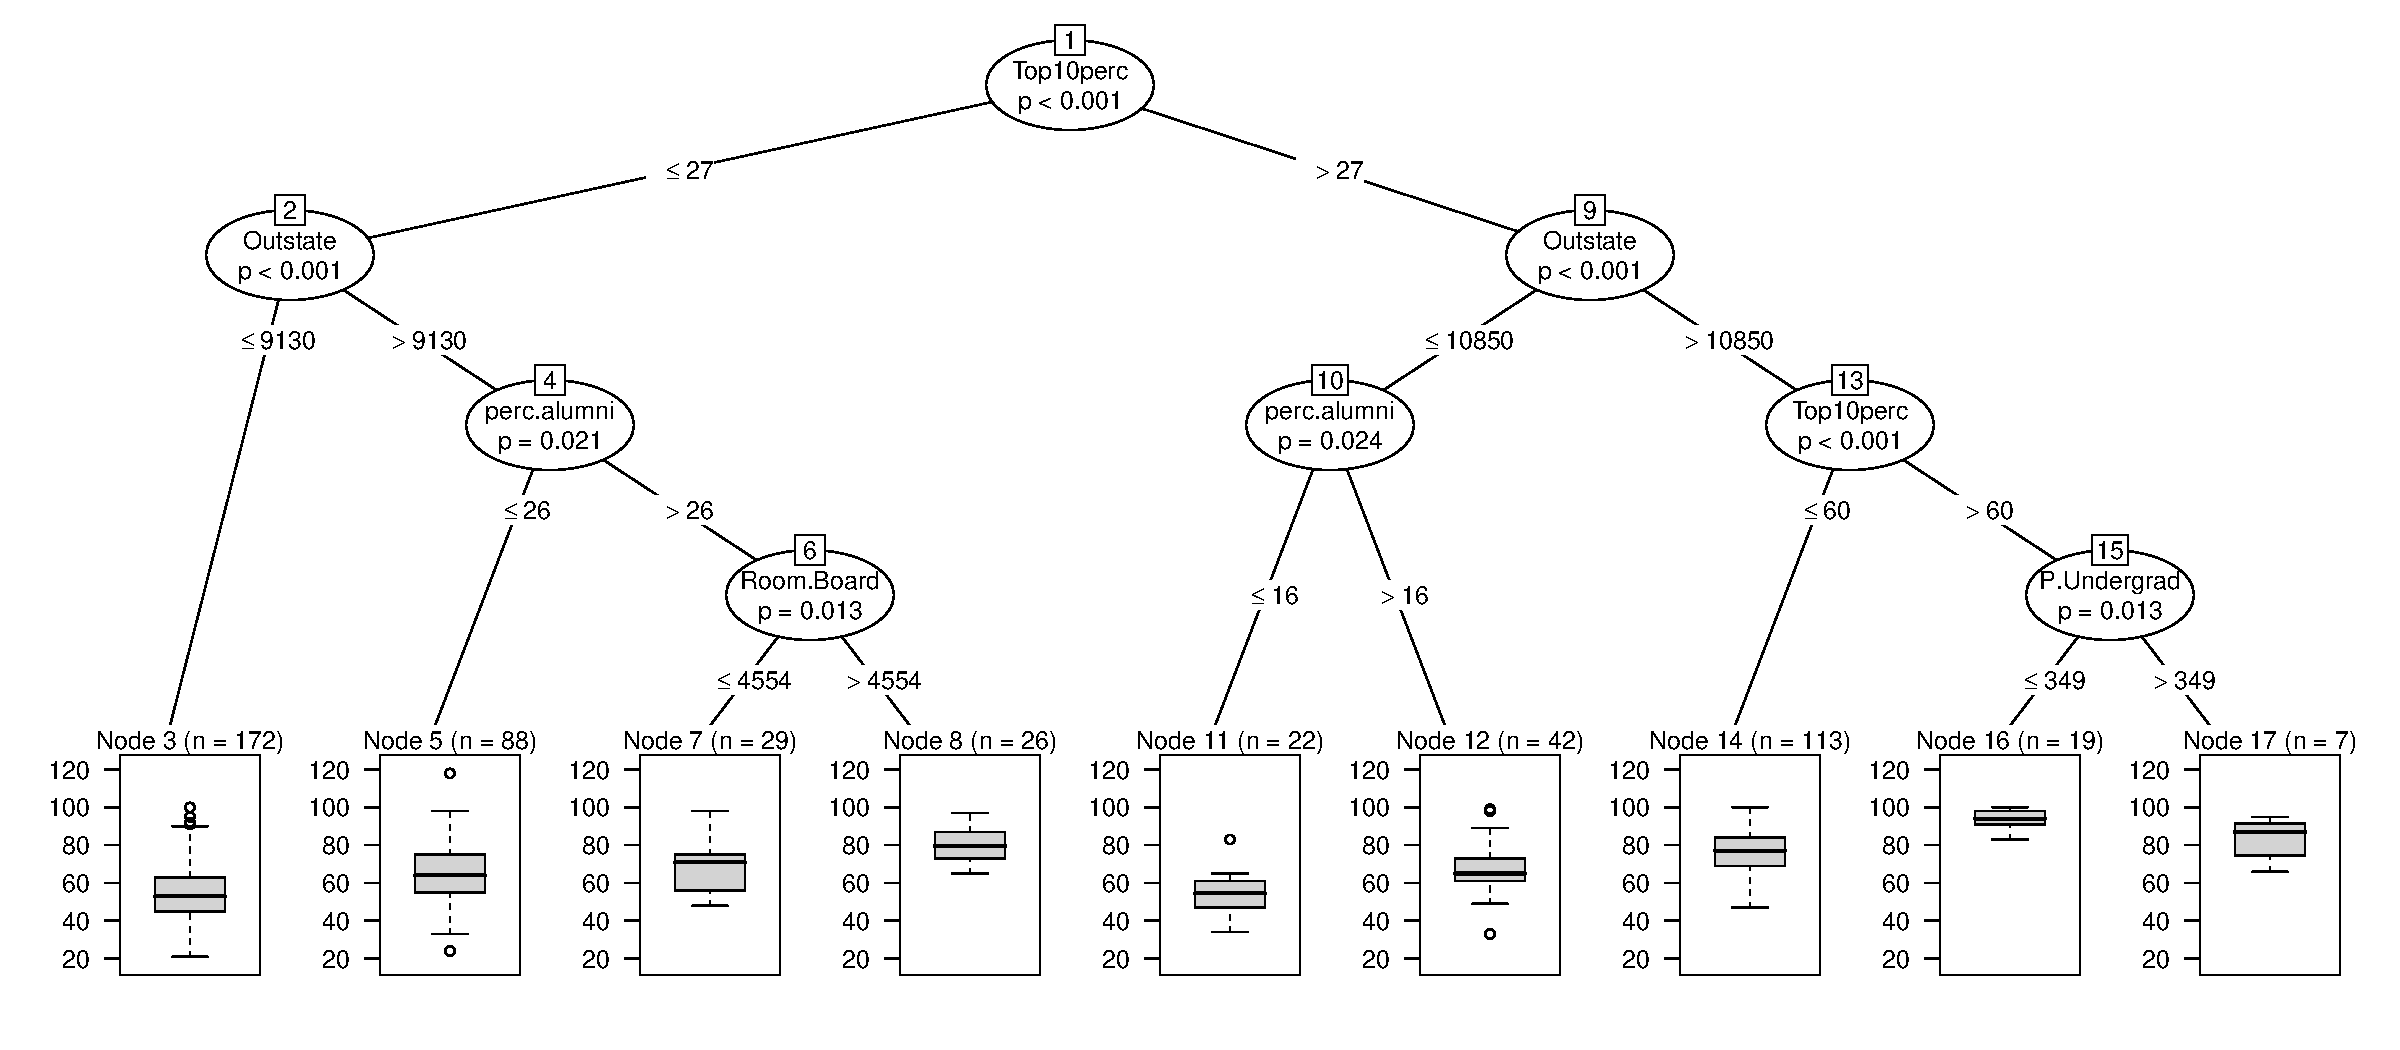
\includegraphics[width = 4.5in]{Figures/Chapter02/ci_tree.pdf}} \\
\subfloat[]{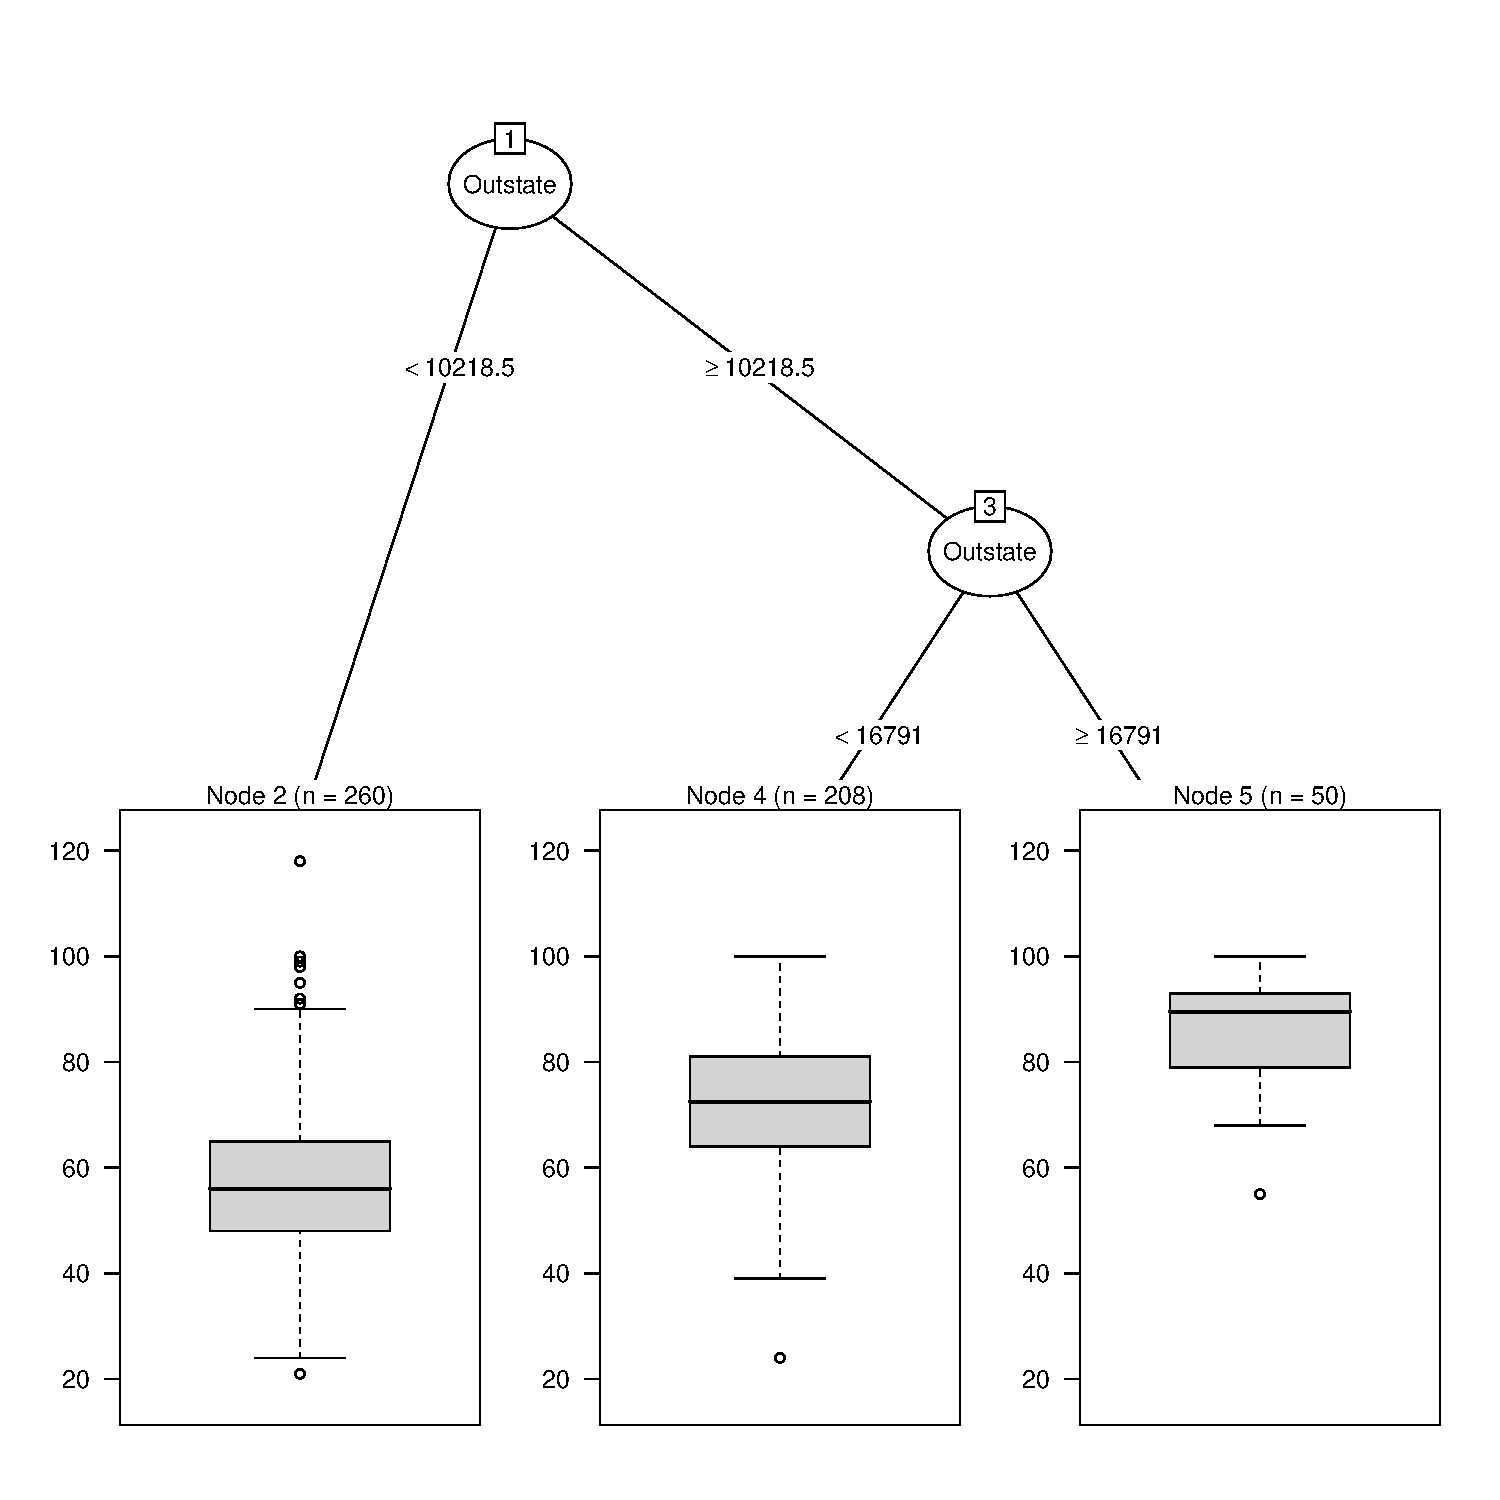
\includegraphics[width = 4.5in]{Figures/Chapter02/cart_tree.pdf}} 
\end{tabular}
\caption[A comparison of a conditional inference tree and a pruned CART tree.]{\textit{A comparison of a conditional inference tree (a) and a pruned CART tree (b). Note that the conditional inference tree contains p-values refering to the significance of each split. Despite a different tree structure, both trees yield similar predictive performance.}}
\label{fig:comparetree}
\end{figure}



%----------------------------------------------------------------------------------------

\subsection{Pros and cons of conditional inference trees}


	Conditional inference trees house all the benefits of decision trees while simultaneously alleviating the issues of both pruning and biased variable selection found in CART. And yet, despite this lack of bias in the splitting procedure, CTREE and CART typically perform similarly with regard to predictive accuracy \cite{hothorn2006unbiased, strobl2007bias}. One downside to this method is that, because it incorporates a permutation framework, the algorithm is much more computationally expensive compared to CART. Thus, if the goal is to simply achieve good predictive accuracy in a tree framework, CART is typically a much better choice. Another major con with the conditional inference framework is that it assumes the data adhere to the traditional assumptions of independence. This potential issue with regard to multilevel data will be discussed further in \autoref{ch:problem}. Finally, like all decision trees, CTREE is a predictive method that is often outperformed by regression techniques. There are two main reasons for this. First, trees are predictive methods that possess high variance. Oftentimes, a small shift in the training set (e.g., sampling the training set more than once) will result in a completely different tree structure being detected \cite{hastie2009elements}. Second, smooth relationships often naturally occur in data sets, and can be better captured with the underlying additive structure found in regression methods compared to the binary, piecewise splits underlying decision trees.


%----------------------------------------------------------------------------------------

\section{Random Forests}


	As mentioned previously, while trees provide intuitive split criteria for a given data set, these decision rules suffer in generalizability performance due to having high variance. \citeA{breiman1996bagging} proposed a solution to this issue by repeatedly taking a bootstrap sample of the training set to create many decision trees, and then aggregating the results of all the trees together to create the final predictions. This technique, referred to as \textit{bagging} (short for bootstrap aggregating), led to better predictive performance due to the fact that trees grown to full length are predictors that have low bias and high variance. Essentially, by aggregating their predictions into an ensemble, this new method maintains the low bias found in single decision trees, but also has reduced variance by replacing the hard, piecewise fits found in decision trees with smoothed relations \cite{breiman1996bagging, buhlmann2002analyzing, strobl2009introduction}.

	One more improvement to this idea was made by \citeA{breiman2001random}. Due to the greediness of the recursive partitioning algorithm, a bagged ensemble of trees is typically dominated by one or two variables that are always used in the first split. This ignores the possibility of the existence of a tree with better predictive performance that contains a first split that is suboptimal. To give these lesser predictors a better chance to be incorporated into the splitting procedure, \citeA{breiman2001random} introduced \textit{random forests}, which first grew decision trees using a random subset of possible predictor values, and then used bootstrap aggregation to create an ensemble. In this method, both the number of variables to select for each tree and the number of trees to grow in total are parameters that can be tuned to yield better predictions. Many statistical software packages have sensible defaults for these values that typically yield good performance, suggesting that a random forest is a good ``off-the-shelf'' method that does not require as much tuning when compared to other predictive models \cite{strobl2009introduction}.


%----------------------------------------------------------------------------------------

\subsection{Out-of-bag samples}


	In a bootstrap sample, the probability of an observation being selected is $1 - (1 - \frac{1}{n})^n$. As $n \rightarrow \infty$, this value converges to approximately 0.632. Thus, by nature of the bootstrap process, approximately 63\% of the data set will be used for training in each decision tree. This highlights a nice feature of random forests, in that about 37\% of the data, referred to as the out-of-bag (OOB) sample, are not used in any given tree. Using the OOB samples to evaluate performance has been shown to be a good approximation of the error found in a separate test set \cite{hastie2009elements}, and are typically used as a replacement for the cross-validation step found in decision trees.


%----------------------------------------------------------------------------------------

\subsection{Variable importance}


	Because random forests include many trees, each with their own distinct set of decision rules, they inevitably become harder to interpret. However, both numerical and graphical methods do exist. One such method is known as \textit{variable importance}, and is typically measured in a permutation framework. More specifically, once an ensemble method has been created, the OOB samples are used to estimate predictive performance. Then, the same data is permuted with respect to a given variable in order to break that variable's link with the outcome, and the predictive accuracy of the overall forest is measured again. Finally, variables are assigned a value that corresponds to the difference in the original prediction accuracy and the permuted prediction accuracy. If the difference is large, then this indicates that the particular variable plays a more important role in predicting the outcome. Otherwise, if the predictive accuracy does not change very much, then this variable does not play a large role in predicting the outcome. See \autoref{fig:varimp} for the variable importance plot for the college graduation rate example. This plot confirms what was found in the single decision tree: out-of-state tuition is the most important variable for predicting college graduation rate.


\begin{figure}[h]
  \centering
  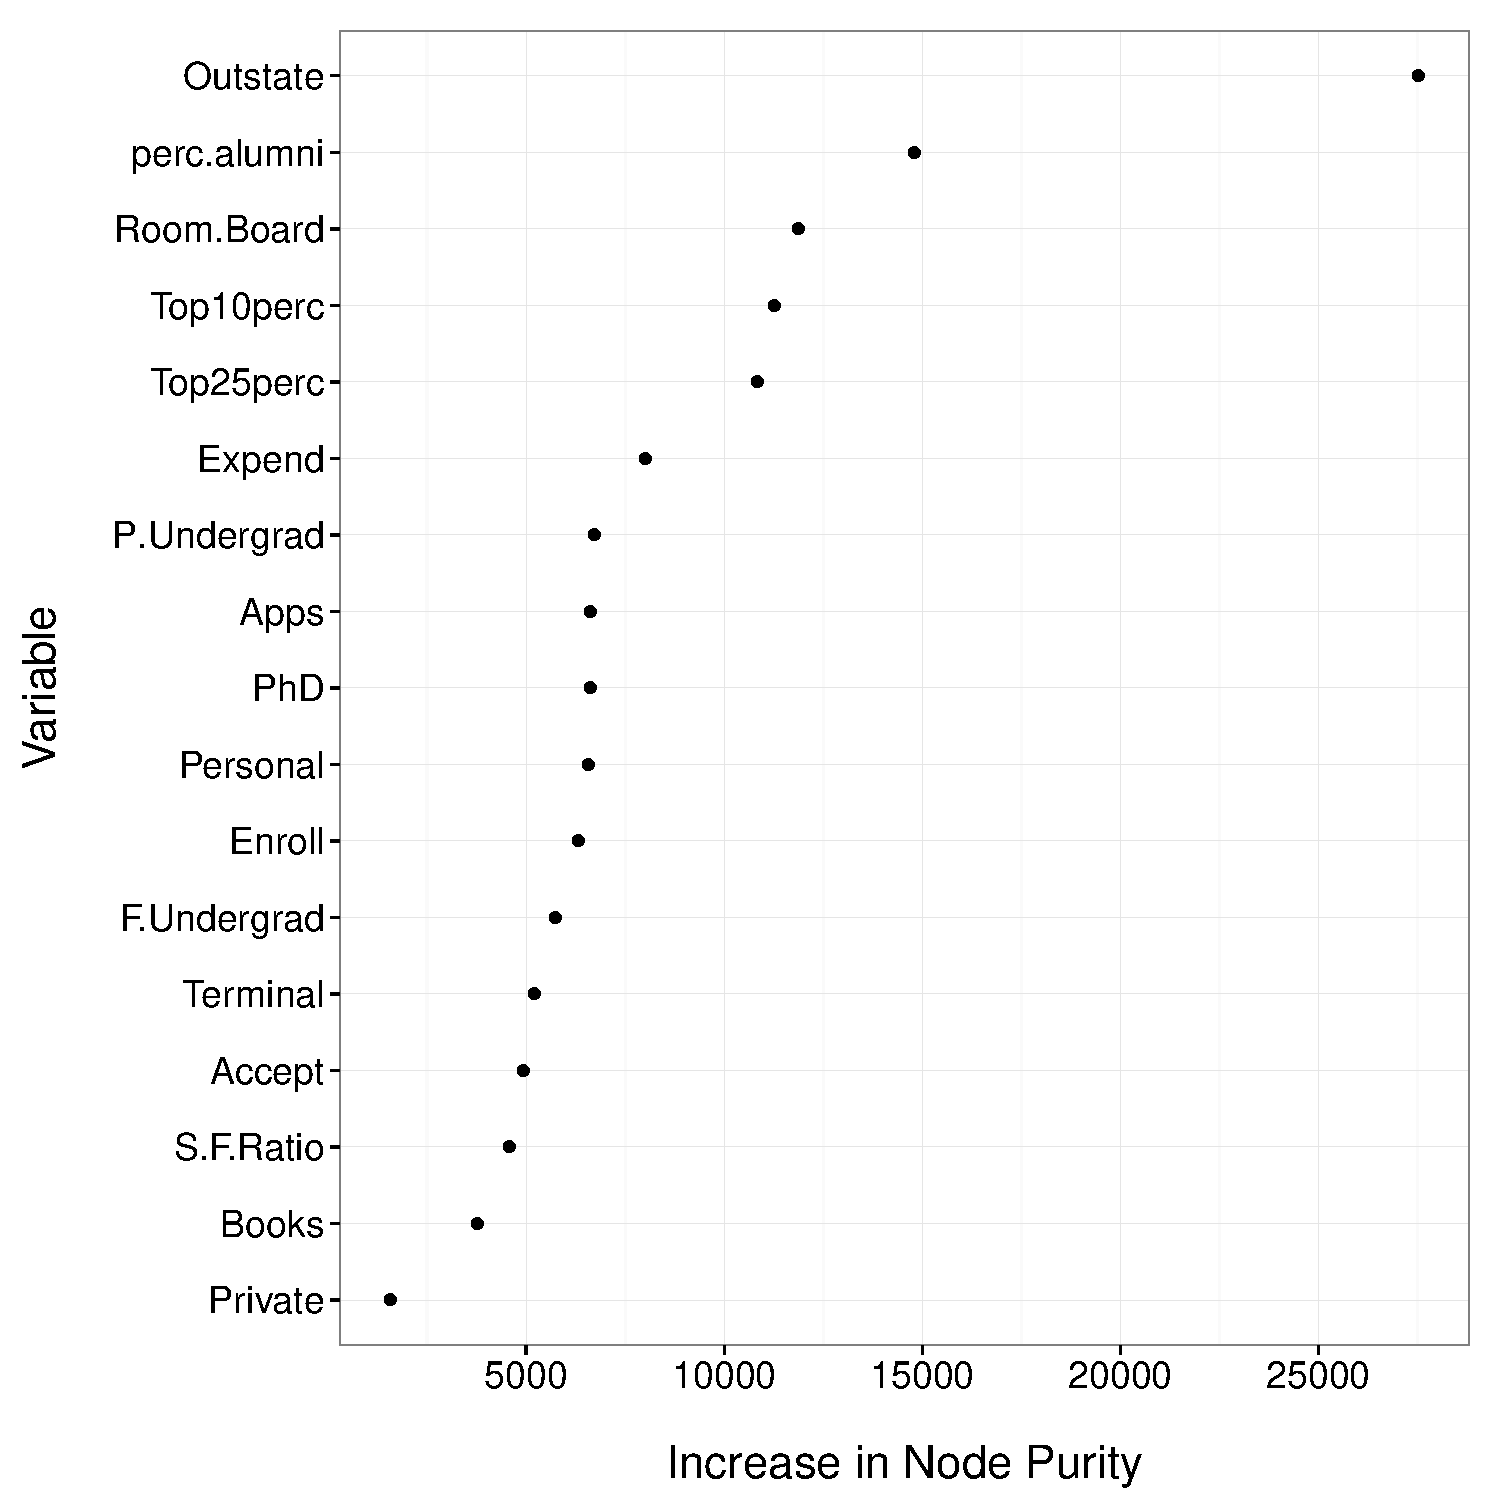
\includegraphics[width=3.5in]{Figures/Chapter02/var_imp_plot.pdf}
  \caption[Variable importance for a CART random forest.]{\textit{Variable importance for a CART random forest, indicating the out-of-state tuition has the largest role in predicting graduation rate.}}
  \label{fig:varimp}
\end{figure}


%----------------------------------------------------------------------------------------

\subsection{Partial dependence plots}


	While variable importance metrics are useful, the functional relations between the variables and the outcome remain hidden from view. One way to further investigate these relations is with \textit{partial dependence plots}. These plots are graphical visualizations of the marginal effect of a given variable (or multiple variables) on an outcome. Typically, these are restricted to only one or two variables due to the limits of human perception, and thus may be misleading due to hidden higher-order interactions. Despite this, partial dependence plots can still be extremely useful for knowledge discovery in large data sets, especially when the random forest is dominated by lower-order interactions and main effects. 


	Following the notation of \citeA{hastie2009elements}, partial dependence plots can be mathematically defined as follows. Suppose $S$ is a subset of $p$ predictor variables, such that $S \subset \left\{X_1, X_2, \ldots, X_p\right\}$. Let $C$ be a complement to $S$, such that $S \cup C = \left\{X_1, X_2, \ldots, X_p\right\}$. The random forest predictor function, $f(X)$, will depend upon all $p$ predictor variables. Thus, $f(X) = f(X_S, X_C)$. The partial dependence of the $S$ predictors on the predictive function $f(X)$ is


\begin{equation}
f_S(X_S) = \mathbb{E}_{X_C}[f(X_S, X_C)]
\end{equation}


\noindent and can be estimated by


\begin{equation}
\bar{f}_S(X_S) = \frac{1}{N}\sum_{i = 1}^{N}[f(X_S, X_{Ci})]
\end{equation}


\noindent where $\left\{x_{C1}, x_{C2}, \ldots, x_{CN}\right\}$ are the values of $X_C$ ocurring over all observations in the training data. In other words, in order to calculate the partial dependence of a given variable (or variables), the entire training set must be utilized for every set of joint values in $X_S$. As one can image, this can be quite computationally expensive when the data set becomes large. See \autoref{fig:partial_dependence} for examples of partial dependence plots for the college graduation rate data set. 

\begin{figure}
\begin{tabular}{c}
\subfloat[]{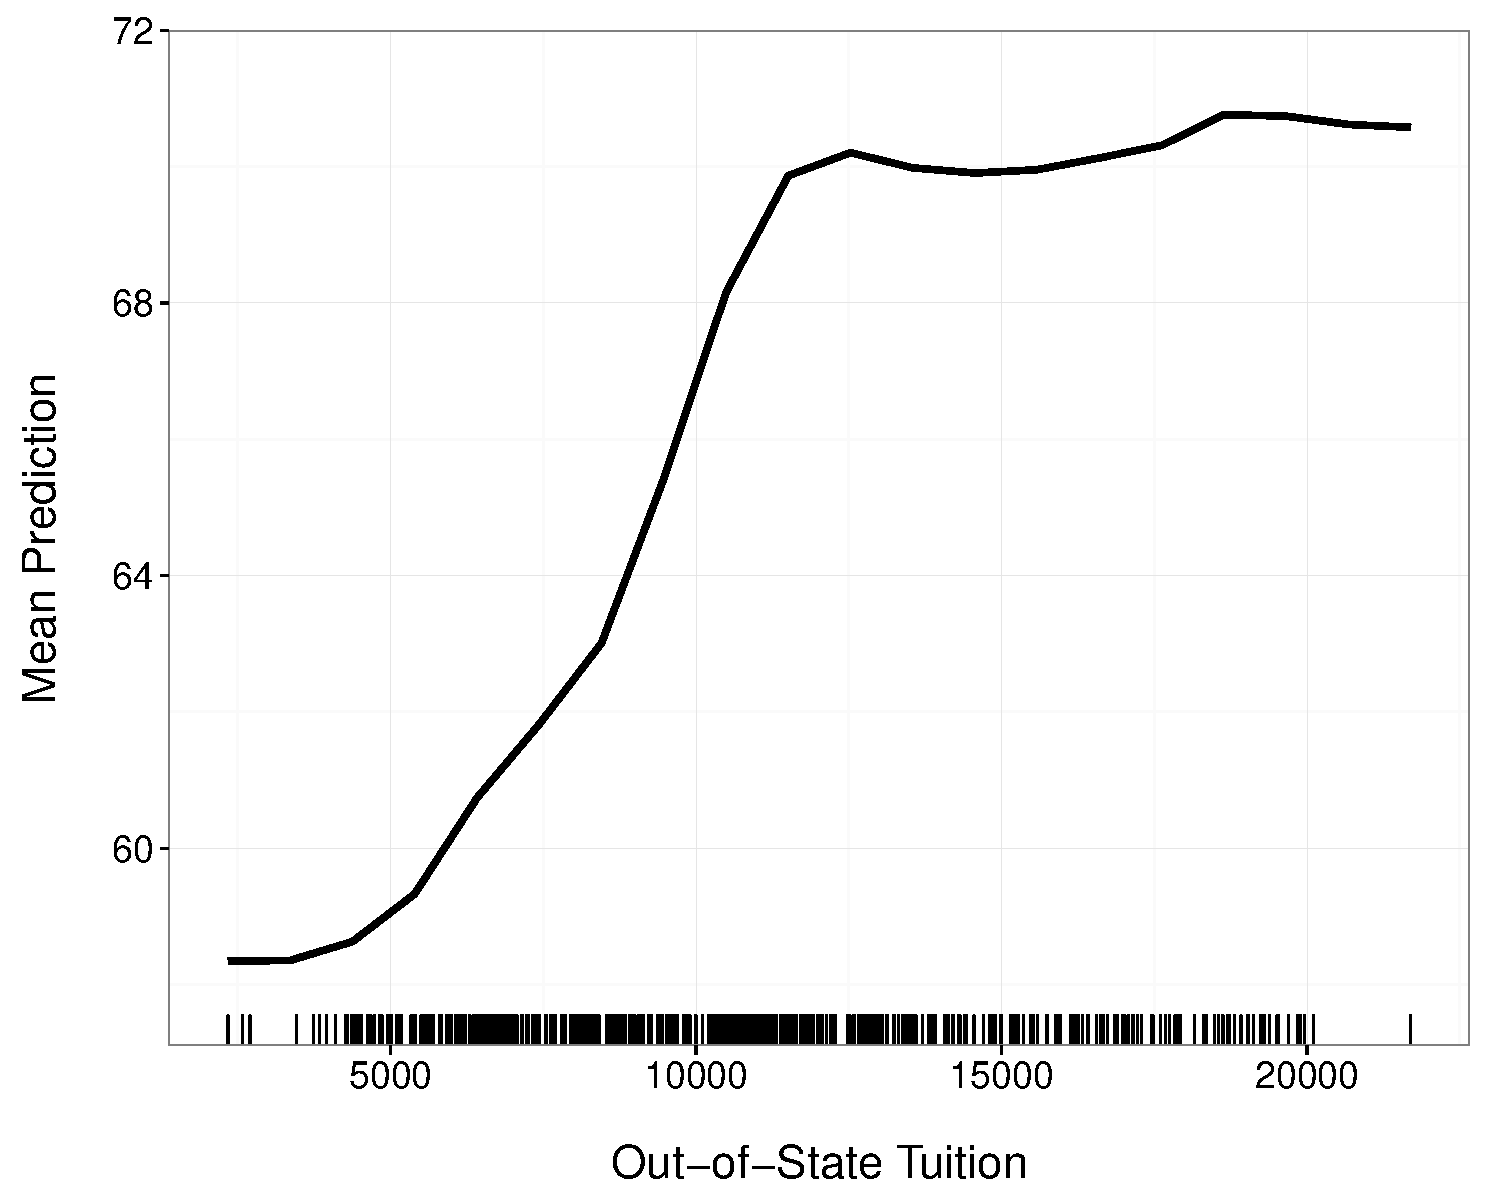
\includegraphics[width = 3.5in]{Figures/Chapter02/part_dep_Outstate.pdf}} \\
\subfloat[]{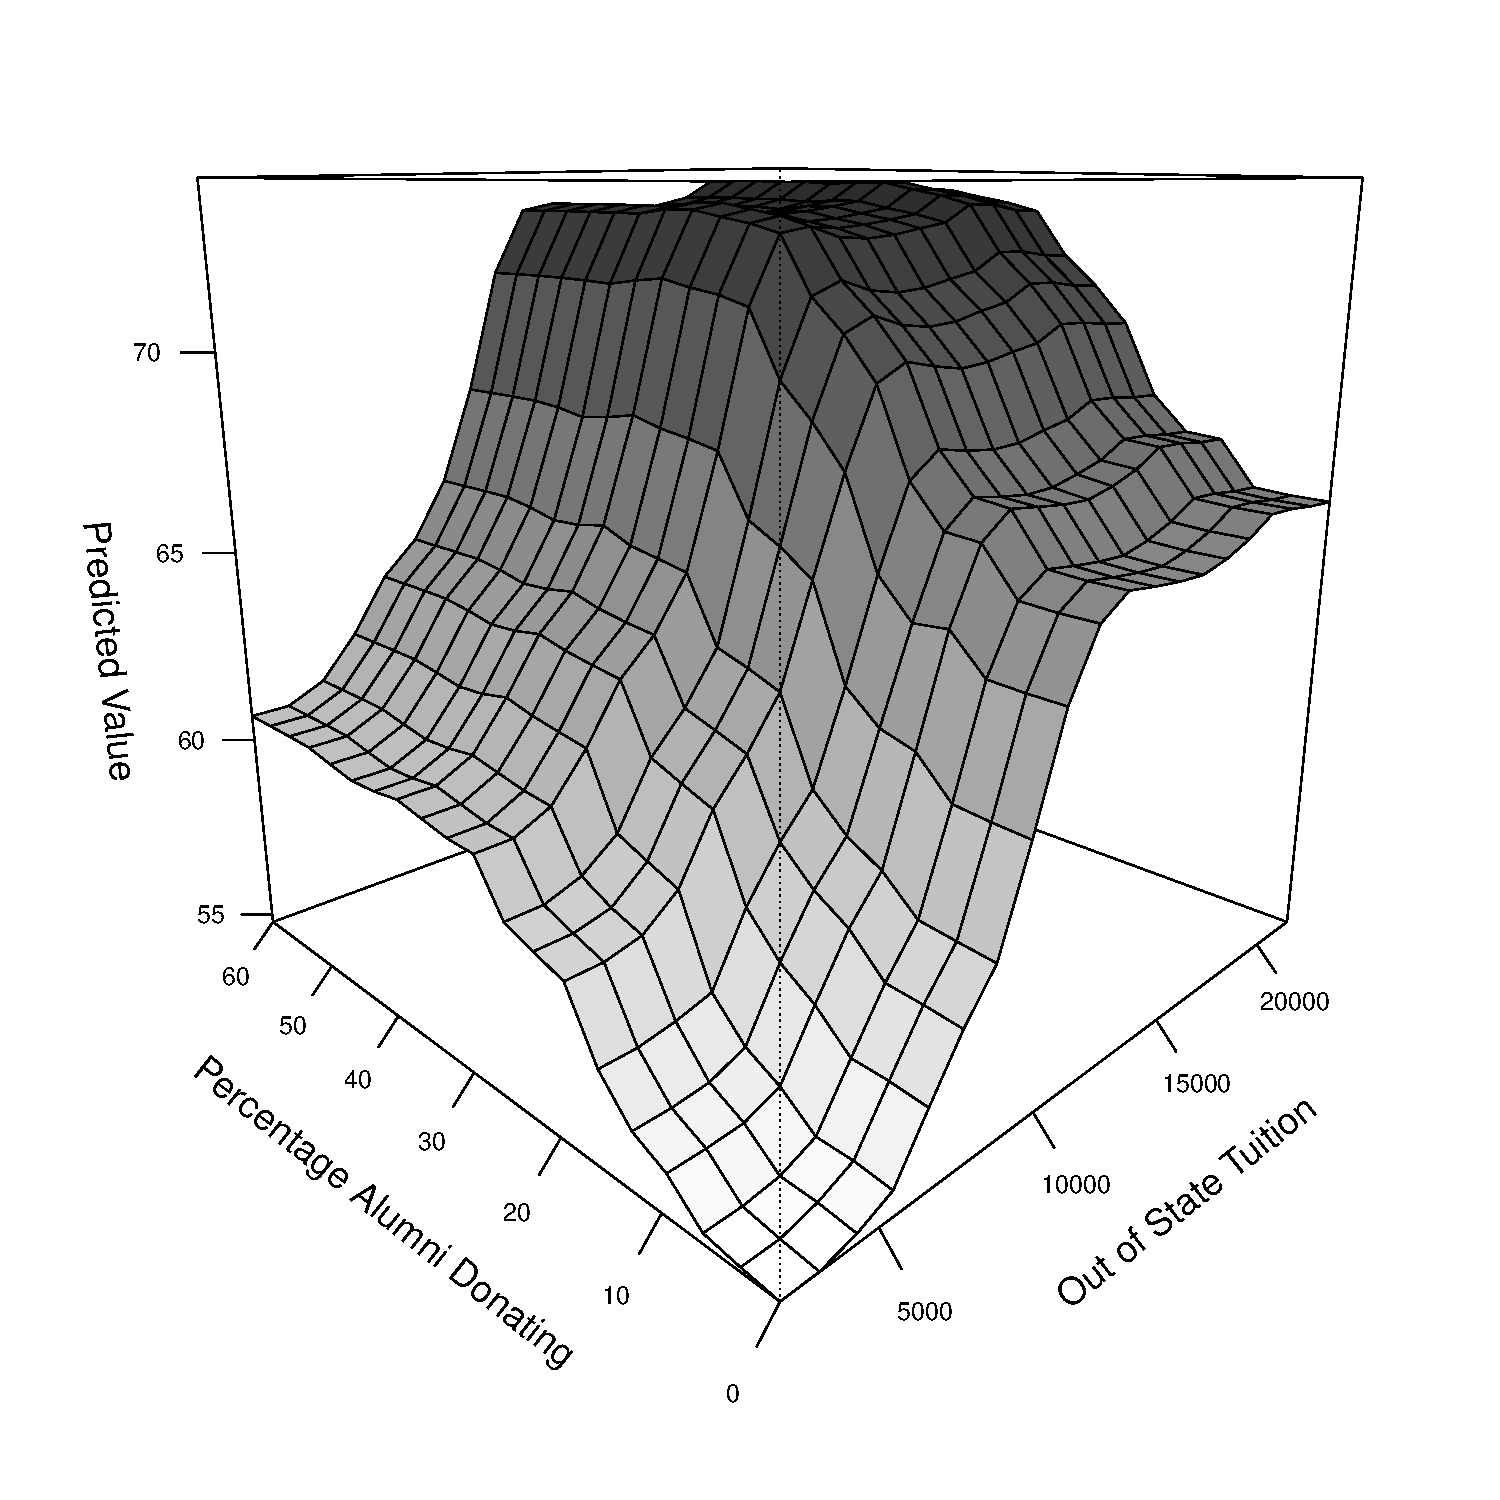
\includegraphics[width = 3.5in]{Figures/Chapter02/plot_3d.pdf}} 
\end{tabular}
\caption[Partial dependence plots for the graduation rate data.]{\textit{(a) shows the partial dependence plot for out-of-state tuition, revealing a somewhat linear relation with graduation rate. (b) shows the partial dependence plot between both out-of-state tuition and percent of alumni donating to the institution, resulting in a three-dimensional plot. Note that because both variables have consistent relations with graduation rate across the values of the other variable, there is no substantial evidence for a potential interaction.}}
\label{fig:partial_dependence}
\end{figure}


	Another visualization tool, similar to partial dependence plots, involves examining how well the predicted relation determined by the random forest approximates the true relation found in the test set. \autoref{fig:testcheck} in one such example, comparing the predicted relation and actual relation for the out-of-state tuition variable. Again, like the partial dependence plot, this is typically performed on the most important predictors to better understand the performance of the random forest, and highlight where the random forest might be doing a poor job.


\begin{figure}[h]
  \centering
  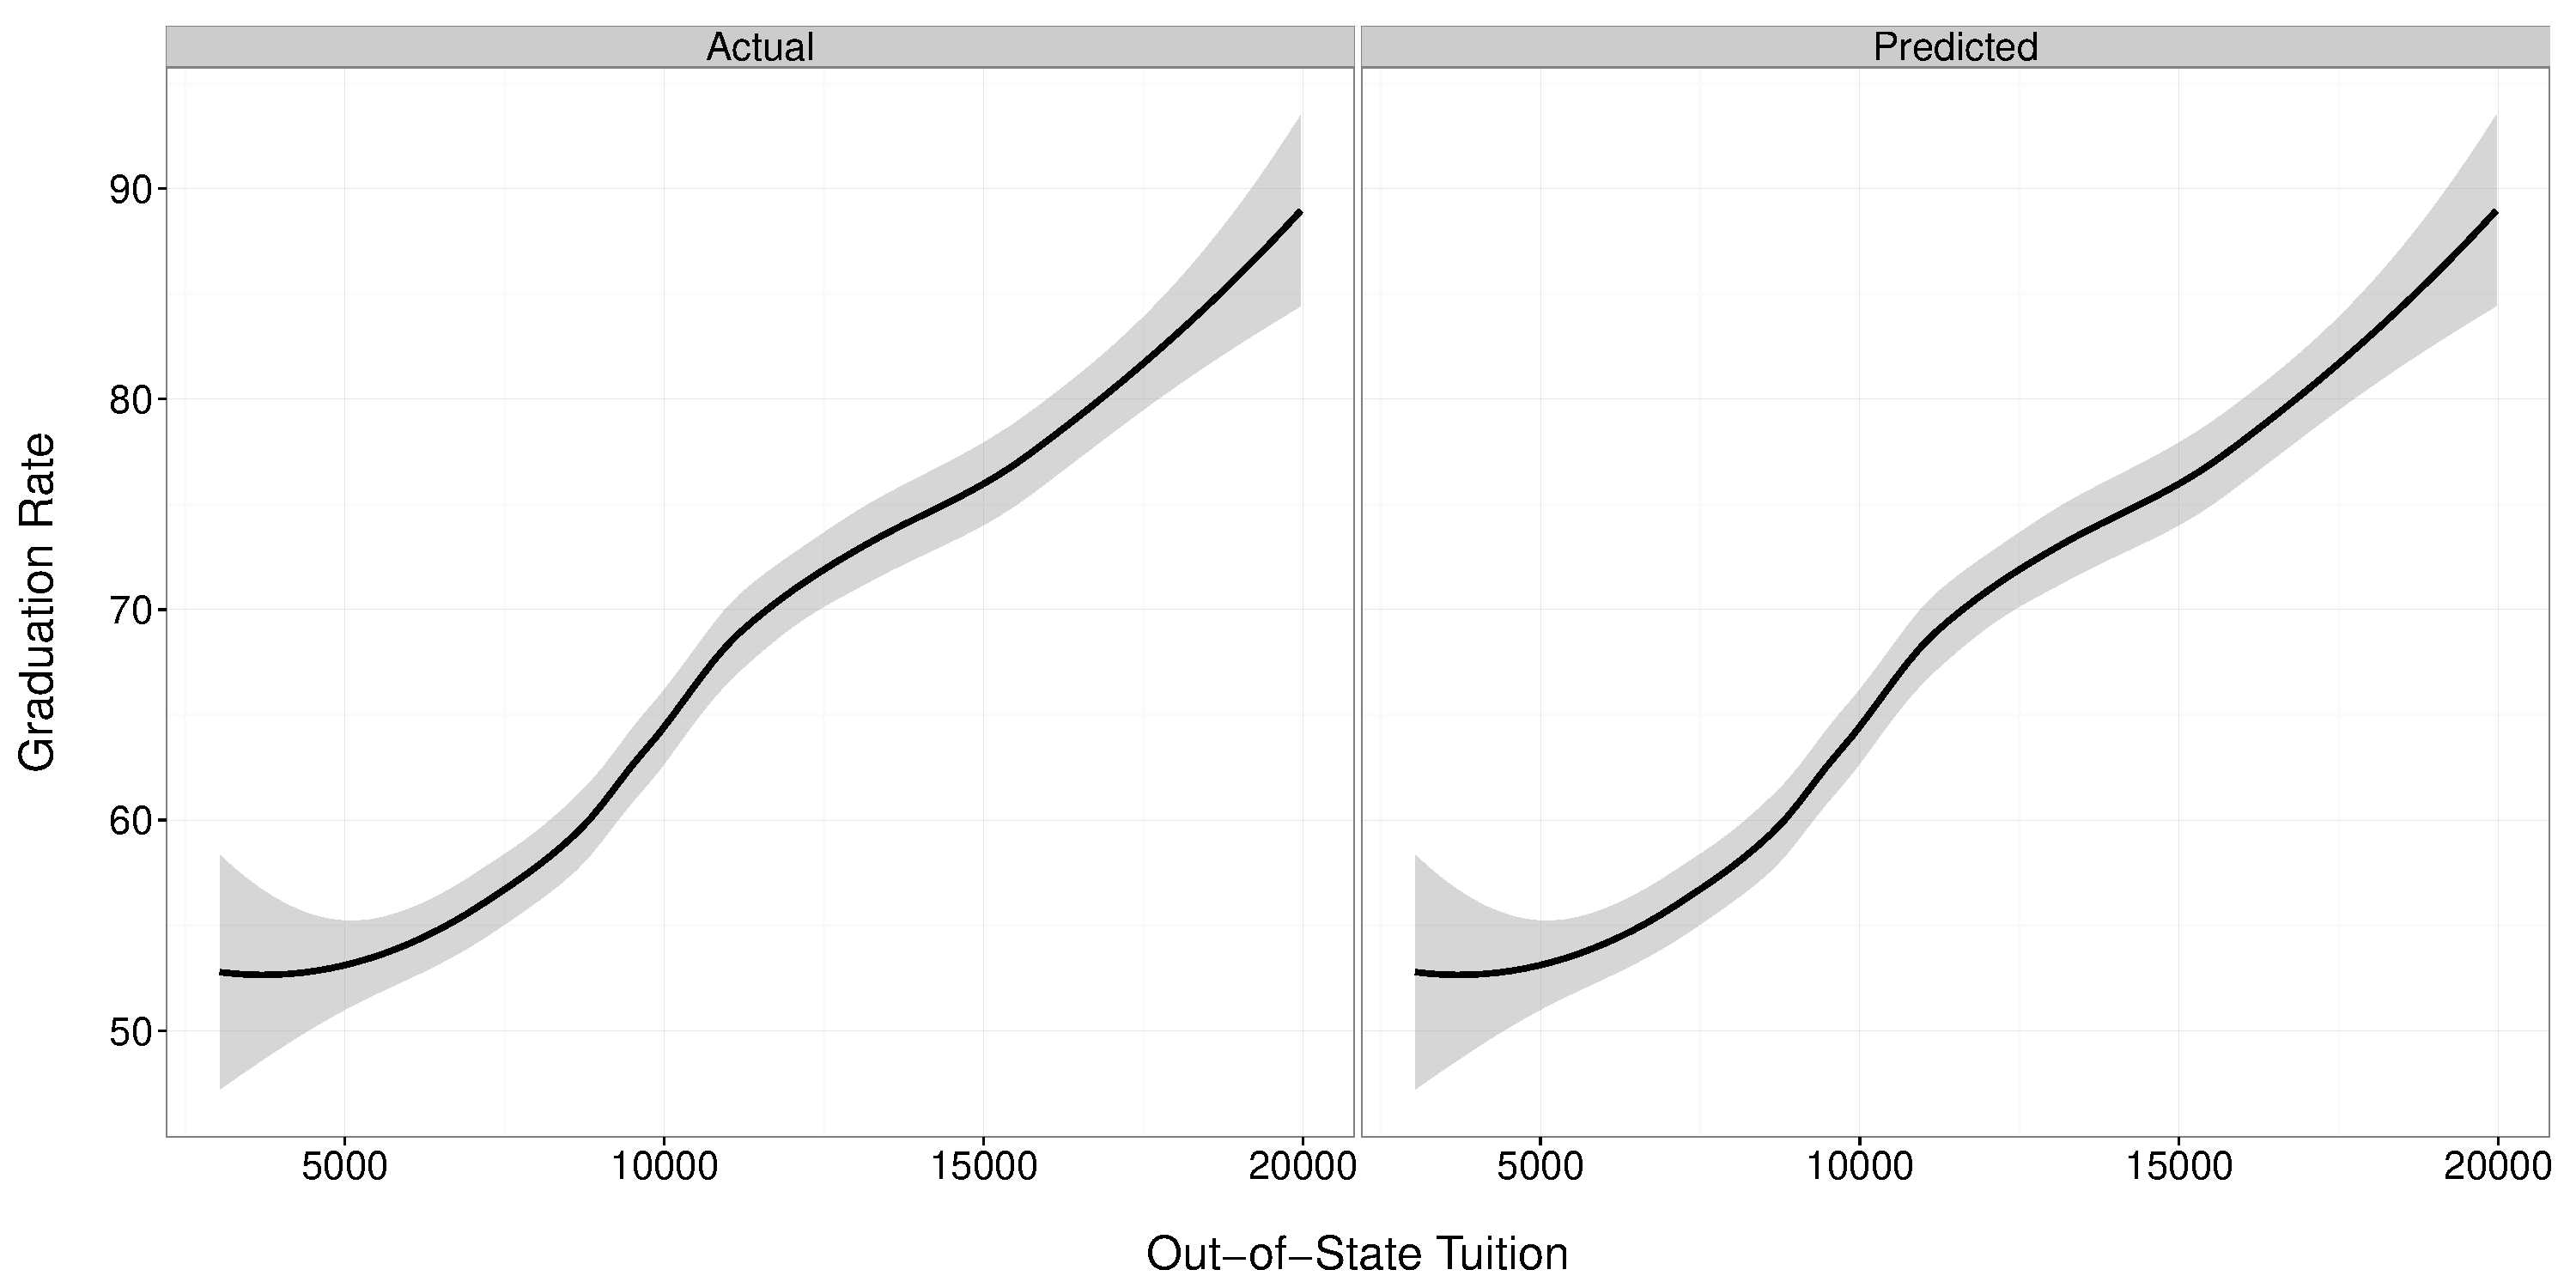
\includegraphics[width=4.5in]{Figures/Chapter02/testcheck_plot.pdf}
  \caption[Comparing the actual relation between out-of-state tuition with the relationship that was predicted with the random forest model.]{\textit{Plot comparing the actual relation between out-of-state tuition (left) with the relation that was predicted from the random forest model (right). In this case, the random forest is doing an excellent job at approximating the true functional form.}}
  \label{fig:testcheck}
\end{figure}



%----------------------------------------------------------------------------------------

\subsection{Conditional inference forests}

	In this overview so far, only a random forest with CART as the underlying partitioning algorithm has been used. In fact, random forests are easily generalizable to any recursive partitioning framework. In the case of conditional inference, for example, creating an ensemble of conditional inference trees is known as a conditional inference forest \cite<CFOREST;>{hothorn2006survival}, and can be readily adapted with one slight alteration to the original forest algorithm. Because the framework of conditional inference assumes independence, taking a bootstrap sample results in a new data set with repeated observations, thus breaking this assumption. In order to maintain an unbiased splitting procedure, this issue can solved by sampling 63.2\% of the data without replacement instead of bootstrapping (i.e., subsampling). This improvement has shown to yield an unbiased splitting procedure with predictive performance on par with CART forests \cite{strobl2007bias}. While the graphical results of the conditional inference forest will not be given for brevity, see \autoref{tab:performance} to compare the predictive performance of CART, CTREE, CART forests, and CFOREST applied to the college graduation rate data in 100 runs. Given the results of CART in \autoref{fig:tradeoff}, the tuning parameter was selected via the minimum cross-validated error rather than the 1-SE rule. Note that the performance for both trees and forests are similar between the two methods of CART and conditional inference. While this is generally true, the underlying decision tree structure will be somewhat different given the biased nature of the CART algorithm \cite{hothorn2006unbiased, strobl2007bias}. In this specific example, the top 5 predictors and their relative order (with the exception of one variable) between both random forest methods were identical.


\begin{table}
\caption[Estimated prediction performance for the four methods]{\textit{Estimated prediction performance for the four methods.}}  
\label{tab:performance}
\begin{tabular}{rcc}
\hline
Method      & Mean Performance (MSE) & SD Performance \\ \hline
CART        & 208.41                 & 19.22          \\
CTREE       & 205.28                 & 17.44          \\
CART forest & 168.61                 & 14.55          \\
CFOREST     & 169.27                 & 14.63          \\ \hline
\end{tabular}
\end{table}


%----------------------------------------------------------------------------------------

\subsection{Pros and cons of Random Forests}


	As was just shown, the major benefit to creating an ensemble of decision trees with a random forest algorithm is being able to efficiently search a large parameter space and create a predictive model that is vastly superior to single decision trees. Another added benefit is that forests are created on unpruned trees, removing the subjectivity inherently found in pruning decisions. However, this benefit of improved performance does come at the cost of reduced interpretability. While both variable importance and partial dependence plots offer ways to view the underlying structure of decision trees, these methods still mask the potential higher-order interactions underlying a given forest that are impossible to visualize. Additionally, forest methods are more computationally expensive to perform when compared to a single decision tree. This is especially true of CFOREST, which requires a more expensive permutation test framework. For example, a recent application of random forests on 876 observations with 44 variables reported 4.82 seconds for CFOREST, while CART forests only took 0.24 seconds \cite{strobl2007bias}. While this effect can be somewhat mitigated on larger data sets by the fact that forests are trivially parallelizable, this characteristic of longer computation time can be perceived as a nuisance, especially with extremely large data sets. 


%----------------------------------------------------------------------------------------

\section{Handling missing data}


	Missing data are an all-too-common occurrence in many areas of the social sciences, especially in education. Fortunately, recursive partitioning has an elegant way to handle missing data, called surrogate splits. Every time a split is made in the procedure, the algorithm automatically searches for additional variables that mimic the behavior of this main split, thus acting as a surrogate to the original variable in the case of a missing observation. These splits are derived in the exact same way as the original partitioning algorithm \cite{hothorn2006unbiased, therneau2014introduction}. More specifically, the algorithm searches for splits in other variables that best predicts membership into the two new classes created by the split in the original variable. A list of ranked variables is then created for each split in the final decision tree in case data are missing on multiple variables. While this approach seems simple, surrogate splits have been shown to yield performance similar to multiple imputation when applied to both CART and CTREE under missingness conditions that are completely at random \cite{hapfelmeier2012recursive}.


	Unfortunately, while the application of the methodology of surrogate splits can extend directly to ensembles of trees for the purpose to calculating predictions, there is no clear way to estimate permuted variable importance in the traditional way. This is one reason as to why surrogate splits are not employed in many CART forest algorithms \cite<e.g.,>{liaw2002classification, pedregosa2011scikit}. Instead, random forests often use imputation methods. For example, the original random forest algorithm employs an imputation method that iteratively builds random forests in order to impute missing values \cite{breiman2001random}. To do this, missing values are first replaced by the median of that variable (in the continuous case) or the category with the highest prevalence (in the categorical case) of that particular variable. Then, a random forest is run, and the missing values are replaced based on their proximity to other observations. That is, when a missing value is present, observations are identified that typically appear in the same nodes as this missing value in many of the trees created during the random forests process. These observations are then used to impute the missing values. This procedure is repeated a few times to iteratively improve on the final imputations. This method has also been shown to yield good performance even with higher rates of missingness (i.e., > 50\%), though it has been noted that the OOB error estimate tends to be slightly optimistic with imputed values \cite{breiman2003manual}. Note that this method only works when covariates are missing, however. Observations with the outcome missing must be either removed or imputed with a separate process.


	CFOREST utilizes surrogate splits and employs a new variable importance measure to allow the estimation of variable importance in the presence of missing data \cite{hapfelmeier2014new}. This new measure is essentially identical to permuted variable importance, with one exception. Rather than randomly permuting a variable to break its link with the outcome, observations are randomly sent to either the left of the right child node of any split that includes the variable of interest. This still breaks a variable's link with the outcome, but now the calculation of variable importance can be accomplished as before. This new technique shows a number of desirable properties over MCAR, MAR, and NMAR data, such as not yielding artificially inflated variable importance values for variables with high rates of missingness, which can occur with complete case analysis \cite{hapfelmeier2014new}. 


%----------------------------------------------------------------------------------------

\section{Other predictive methods}

	Note that recursive partitioning was specifically chosen as the focus of this dissertation given that it is nonparametric in nature, relatively easy and intuitive to understand, and their ensemble method counterparts (i.e., forests) consistently shows good performance in predictive tasks when compared to other popular methods \cite{caruana2006empirical}. However, these methods are certainly not a ``silver bullet'' for exploratory data analysis or predictive modeling in general. For example, while recursive partitioning will estimate potential non-linear relationships, linearity is often a valid assumption to make in many statistical applications. Regularized regression methods that include a penalty term in its estimation procedure, such as the L2 norm (i.e., the sum of the squared, standardized parameter estimates) in the case of ridge regression or the L1 norm (i.e., the sum of the absolute value of the standardized parameter estimates) in the case of the LASSO, can be attractive options to reduce overfitting in linear models at the small cost of increased bias \cite{hastie2009elements}. Still, extending these methods into a mixed-effects framework is a much more complicated task given the underlying assumptions of regression models, though some solutions do exist \cite<e.g.,>{eliot2011ridge, schelldorfer2011estimation}.







